\documentclass[%
paper=a4,       % Papiergröße
fontsize=11pt,  % Schriftgröße
ngerman         % Option für deutsche Sprache
]{scrreprt}
\usepackage{scrhack}
%\documentclass[%
%paper=a4,       % Papiergröße
%fontsize=12pt,  % Schriftgröße
%ngerman         % Option für deutsche Sprache
%]{scrreprt}

% Basics für Codierung und Sprache
% ===========================================================
\usepackage{framed}
\usepackage{lipsum}
\usepackage[final]{graphicx}          % Einbindung von Grafiken
\graphicspath{{figs/}}
\usepackage{subcaption}
\usepackage{babel}                    % deutsche Silbentrennung, etc.
\usepackage[german=quotes]{csquotes}  % deutsche Anführungszeichen mit \enquote{...}
\usepackage{titling}
\usepackage{booktabs} % für tabellen
\RequirePackage[backend=biber, style=numeric]{biblatex}     % erlaubt das Einfügen eines Quellenverzeichnisses
% ===========================================================

% Fonts und Typographie
% ===========================================================
%\usepackage{sourcecodepro}
\usepackage[T1]{fontenc}
%\usepackage{lmodern}
%\usepackage{mathptmx}
\usepackage{mathpazo} % Palatino
%\usepackage{helvet} % Helvetica
%\usepackage{courier} % Courier
%\usepackage{times}
\usepackage{fix-cm}
\usepackage{anyfontsize}
%\usepackage[default]{sourcesanspro}
%\usepackage{nimbusmononarrow}

\usepackage[babel=true,final,tracking=smallcaps]{microtype}
\DisableLigatures{encoding = T1, family = tt* }   % keine Ligaturen für Monospace-Fonts
% ===========================================================

% Farben
% ===========================================================
\usepackage[x11names]{xcolor}
% ===========================================================

% Mathe-Pakete und -Einstellungen
% ===========================================================
%\usepackage{yhmath}
\usepackage{amsmath}
\usepackage{amsthm}
\usepackage{mathtools}             % Tools zum Setzen von Formeln
\usepackage{amssymb,}               % übliche Mathe-Symbole
\usepackage[bigdelims]{newtxmath}  % moderne Mathe-Font
\allowdisplaybreaks                % seitenübergreifende Rechnungen
\usepackage{bm}                    % math bold font
\usepackage{wasysym}               % noch mehr Symbole
\usepackage{siunitx}
\sisetup{output-decimal-marker = {,}} % Kommas als Dezimalteiler
\DeclareSIUnit\barn{b}
% ===========================================================

% TikZ
% ===========================================================
\usepackage{tikz}
\usetikzlibrary{arrows,arrows.meta}   % mehr Pfeile!
\usetikzlibrary{calc}                 % TikZ kann rechnen
\usetikzlibrary{positioning}
\tikzset{>=Latex}                     % Standard-Pfeilspitze
% ===========================================================

% Seitenlayout, Kopf-/Fußzeile
% ===========================================================
\usepackage[bottom=3cm, left=2.5cm, right=2cm]{geometry}
\RequirePackage[headsepline]{scrlayer-scrpage} % edit header and footer of a page, for more lines add [headtopline, headsepline, footsepline, footbotline]
\pagestyle{scrheadings} % set formatting to scrheadings
\clearpairofpagestyles
\setkomafont{pageheadfoot}{}

% ===========================================================

% Hyperref für Referenzen und Hyperlinks
% ===========================================================
\usepackage[%
hidelinks,
pdfpagelabels,
bookmarksopen=true,
bookmarksnumbered=true,
linkcolor=black,
urlcolor=SkyBlue2,
plainpages=false,
pagebackref,
citecolor=black,
hypertexnames=true,
pdfborderstyle={/S/U},
linkbordercolor=SkyBlue2,
colorlinks=false,
backref=false]{hyperref}
\hypersetup{final}
\usepackage{cleveref}
\crefname{figure}{Abb.}{Abb.}
\crefname{table}{Tab.}{Tab.}
\crefname{equation}{Gl.}{Gl.}
% ===========================================================

% Listen und Tabellen
% ===========================================================
\usepackage{multicol}
\usepackage[shortlabels]{enumitem}
\setlist{itemsep=0pt}
\setlist[enumerate]{font=\sffamily\bfseries}
\setlist[itemize]{label=$\triangleright$}
\usepackage{tabularx}
% ===========================================================

% listings
% ===========================================================
\usepackage{listingsutf8}
\lstset{
	belowcaptionskip=1\baselineskip,
	breaklines=true,
	showstringspaces=false,
	basicstyle=\ttfamily,
	keywordstyle=\bfseries\color{green!40!black},
	commentstyle=\itshape\color{purple!40!black},
	stringstyle=\color{orange},
	numbers=left,
	numberstyle=\footnotesize\ttfamily\color{gray},
	inputencoding=utf8/latin1,
	tabsize=4,
}

%%%%%%%%%%%%%%%%%%%%%%%%%%%%%%%%%%%%%%%%%%%%%%%%%%%%%%%%%%%
%%% Ab hier folgen nur noch vordefinierte Shortcuts %%%
%%%%%%%%%%%%%%%%%%%%%%%%%%%%%%%%%%%%%%%%%%%%%%%%%%%%%%%%%%%

\newcommand{\BB}{\mathbb{B}}
\newcommand{\CC}{\mathbb{C}}
\newcommand{\NN}{\mathbb{N}}
\newcommand{\QQ}{\mathbb{Q}}
\newcommand{\RR}{\mathbb{R}}
\newcommand{\ZZ}{\mathbb{Z}}
\newcommand{\oh}{\mathcal{O}}

\newcommand{\ol}[1]{\overline{#1}}
\newcommand{\wt}[1]{\widetilde{#1}}
\newcommand{\wh}[1]{\widehat{#1}}

\DeclareMathOperator{\id}{id}                        % Identität
\DeclareMathOperator{\pot}{\mathcal{P}}              % Potenzmenge

% Klammerungen und ähnliches
\DeclarePairedDelimiter{\absolut}{\lvert}{\rvert}    % Betrag
\DeclarePairedDelimiter{\ceiling}{\lceil}{\rceil}    % aufrunden
\DeclarePairedDelimiter{\Floor}{\lfloor}{\rfloor}    % aufrunden
\DeclarePairedDelimiter{\Norm}{\lVert}{\rVert}       % Norm
\DeclarePairedDelimiter{\sprod}{\langle}{\rangle}    % spitze Klammern
\DeclarePairedDelimiter{\enbrace}{(}{)}              % runde Klammern
\DeclarePairedDelimiter{\benbrace}{\lbrack}{\rbrack} % eckige Klammern
\DeclarePairedDelimiter{\penbrace}{\{}{\}}           % geschweifte Klammern
\newcommand{\Underbrace}[2]{{\underbrace{#1}_{#2}}}  % bessere Unterklammerungen

% Kurzschreibweisen für Faule und Code-Vervollständigung
\newcommand{\abs}[1]{\absolut*{#1}}
\newcommand{\ceil}[1]{\ceiling*{#1}}
\newcommand{\flo}[1]{\Floor*{#1}}
\newcommand{\no}[1]{\Norm*{#1}}
\newcommand{\sk}[1]{\sprod*{#1}}
\newcommand{\enb}[1]{\enbrace*{#1}}
\newcommand{\penb}[1]{\penbrace*{#1}}
\newcommand{\benb}[1]{\benbrace*{#1}}
\newcommand{\stack}[2]{\makebox[1cm][c]{$\stackrel{#1}{#2}$}}

%\newcommand{\vector}[1]{%
%\begin{pmatrix} #1 \end{pmatrix}
%}
%==== Enumerationstyle 1.1.1
\renewcommand{\labelenumii}{\arabic{enumi}.\arabic{enumii}}
\renewcommand{\labelenumiii}{\arabic{enumi}.\arabic{enumii}.\arabic{enumiii}}
\renewcommand{\labelenumiv}{\arabic{enumi}.\arabic{enumii}.\arabic{enumiii}.\arabic{enumiv}}
%

\newcommand{\cby}[1]{\colorbox{yellow}{#1}} % yellow colorbox
\newcommand{\cbb}[1]{\colorbox{black}{#1}} % black colorbox



\addbibresource{refs.bib}
%\addfigurepath{figs}

% === Header =======================
\setlength\headheight{24pt}
\setlength\footheight{15pt}
\ihead{\textbf{V401: Elektronische Übergänge in Atomen}}			% inner header
\chead{}						% center header
\ohead{\textbf{\headmark}}		% outer header
\cfoot*{\pagemark}				% center footer
\automark{section}				
\KOMAoptions{headsepline=.4pt:19\textwidth}  % 0.4pt thick line, full width
\renewcommand*\chapterheadstartvskip{\vspace*{-1cm}}

% ==================================

\begin{document}

\begin{titlepage}
\newcommand{\HRule}{\rule{\linewidth}{0.5mm}}
\center{}
\textsc{\LARGE }\\[1.5cm] % Name of your university/college
\textsc{\LARGE Praktikum 4}\\[0.5cm] % Major heading such as course name
\textsc{\large Atome, Moleküle, kondensierte Materie}\\[0.5cm] % Minor heading such as course title

%----------------------------------------------------------------------------------------
%	TITLE SECTION
\HRule{}\\[0.4cm]
{ \huge \bfseries Versuch 401: Elektronische Übergänge\\[0.3cm] in Atomen}\\[0.4cm] % Title of your document
\HRule{}\\[0.2cm]
\Large{\textsc{Gruppe A201}}\\[0.2cm]
 
%----------------------------------------------------------------------------------------
%	AUTHOR SECTION
\begin{minipage}{0.4\textwidth}
\begin{flushleft} \large
\textsc{Parth Gadhavi} % Your name
\end{flushleft}
\end{minipage}
%~
\begin{minipage}{0.4\textwidth}
\begin{flushright} \large
\textsc{Jaffar Al Naggar}
\end{flushright}
\end{minipage}\\[2.0cm]

{\large Versuchsdurchführung\, 28/29. April 2025 }\\[7.9cm] % Date, change the \today to a set date if you want to be precise

%----------------------------------------------------------------------------------------
%	LOGO SECTION

\includegraphics[width=6 cm]{logo.png}\\[1cm] % Include a department/university logo - this will require the graphicx package
 
%----------------------------------------------------------------------------------------

\vfill % Fill the rest of the page with whitespace

\end{titlepage}
\tableofcontents
\clearpage
\clearpage
\setcounter{page}{1}
\chapter{Einleitung}
In Versuch \textit{401: Elektronische Übergängen in Atomen} werden elektronische Übergänge zwischen diskreten Energieniveaus in Atomen anhand zweier experimenteller
Methoden untersucht.
\vspace{0.3cm}\\
Im ersten Versuchsteil wird die Aufspaltung atomarer Spektrallinien im externen Magnetfeld, der \textit{Zeemann}-Effekt, betrachtet. Anhand eines ausgewählten
Übergangs im Cadmium (Cd)-Atom ($5^1D_2 \rightarrow 5^1P_1$) wird die Abhängigkeit der Linienaufspaltung von der Magnetfeldstärke sowie die Polarisationseigenschaften der 
emmittierten Strahlung untersucht. Zur hochauflösenden Darstellung werden ein \texttt{Fabry-Pérot-Etalon} und eine \texttt{CCD-Kamera} verwendet.\\
Im Rahmen der Auswertung werden das \textit{Bohrsche-Magneton} sowie die Finesse und das Auflösungsvermögen des Etalons bestimmt.
\vspace{0.3cm}\\
Der zweite Versuchsteil befasst sicht mit dem  \textit{Franck-Hertz}-Versuch, der die diskrete Energieaufnahme von Atomen bei Elektronenstößen untersucht.\\
Durch Aufnahme der Anodenstrom-Spannungs-Kurve und deren Analyse wird die Anregungsenergie von Quecksilber (Hg)-Atomen ermittelt.\\
Zusätzlich werden die Einflüsse von Temperaturänderung und variabler Gegenspannung auf die Form der Stromkurve untersucht, um die Wechselwirkung zwischen freien Elektronen und Hg-Atomen
unter verschiedenen Bedingungen zu analysieren.
\vspace{0.3cm}\\
Der gesamte Versuch dient dazu, die Quantelung atomarer Eigenschaften experimentell nachzuweisen und daraus charakteristische Größen herzuleiten.
\chapter{Zeemann-Effekt}
Für den Übergang von Cadmium $5^1D_2 \rightarrow 5^1P_1$ wird der normale \texttt{Zeemann}-Effekt untersucht. Dafür folgt zunächst ein theoretischer Einschub.
% -----
\section{Theoretischer Hintergrund}

Der \texttt{Zeemann}-Effekt beschreibt die Aufspaltung von Spektrallinien, und somit Aufhebung der Entartung der Energieniveaus gleicher Gesamtdrehimpulse $J$, in einem externen Magnetfeld. 
Diese Aufspaltung ist auf die Wechselwirkung des magnetischen Moments der Atome mit dem äußeren Magnetfeld zurückzuführen.
Unterschieden wird zwischen dem \textit{normalen} ($S=0$) und dem \textit{anormalen} ($S\neq 0$) \texttt{Zeemann}-Effekt.\\
Da beide Niveaus des Cd einen Gesamtspin von $S=0$ besitzen, ist nur der normale \texttt{Zeemann}-Effekt relevant.
Der Hamiltonian des Elektrons im Atom und im Magnetfeld folgt mit:
%--
\begin{equation}
    \widehat{H}= 
    \underbrace{-\frac{\hbar}{2m}\vec{\nabla}^2 
    -\frac{e^2}{4\pi\varepsilon_0 r}}_{\raisebox{1.5ex}{\scriptsize $H_\mathrm{0}$}} 
    \underbrace{+\beta\frac{\hat{\vec{L}}\cdot\hat{\vec{S}}}{\hbar^2}}_{\raisebox{1.5ex}{\scriptsize $H_{\mathrm{Spin-Bahn}}$}}
    \underbrace{+\mu_B\frac{\hat{\vec{L}}+2\hat{\vec{S}}}{\hbar}\vec{B}}_{\raisebox{1.5ex}{\scriptsize $H_{\mathrm{Zeemann}}$}}
\end{equation}
%--
mit dem \textit{Spin-Bahn}-Kopplungsterm $H_{\mathrm{Spin-Bahn}}$ aus der Feinstruktur und dem \textit{Zeemann}-Kopplungsterm $H_{\mathrm{Zeemann}}$ aus der 
Wechselwirkung mit dem äußeren Magnetfeld mit Richtung $\vec{B}=B\vec{e}_z$.\\
Da jedoch $S=0$ fallen einige Terme weg. Die guten Quantenzahlen, also die, die sich nicht ändern, sind $L$, $S$, $J$ und $M_J$ (wobei $J=L+S=L$) und die 
Energiekorrektur zum Hamiltonian ist:
%--
\begin{equation}
    \Delta E = \mu_B g_J M_J B
\end{equation}
%--
mit dem Bohrschen Magneton $\mu_B = \frac{e\hbar}{2m}$ und dem Landé-Faktor $g_J$:
%--
\begin{equation}
    g_J = 1 + \frac{J(J+1) + S(S+1) - L(L+1)}{2J(J+1)}
\end{equation}
%--
Die Aufspaltung der Energieniveaus und möglichen Übergänge für die verschiedenen $M_J$ anhand der Auswahlregeln
%--
\begin{align*}
    \Delta J &= 0, \pm 1\\
    \Delta M_J &= 0, \pm 1
\end{align*}
%--
sind in \cref{fig:cd_niveaus} dargestellt.
%--
\vspace{0.3cm}\\
Die Polarisation der Strahlung hängt von der Änderung der magnetischen Quantenzahl $M_J$ im Übergang ab (siehe \cref{fig:polarisation}):
%--
\begin{itemize}
    \item \textbf{$\pi$-Übergänge:} $\Delta M_J = 0$ — linear polarisiert parallel zur Magnetfeldrichtung
    \item \textbf{$\sigma^+$-Übergänge:} $\Delta M_J = +1$ — rechtszirkular polarisiert (bei longitudinaler Beobachtung)
    \item \textbf{$\sigma^-$-Übergänge:} $\Delta M_J = -1$ — linkszirkular polarisiert (bei longitudinaler Beobachtung)
\end{itemize}
%--
Je nach Beobachtungsrichtung relativ zum Magnetfeld lassen sich unterschiedliche Polarisationen der emittierten Strahlung beobachten:
%--
\begin{itemize}
    \item \textbf{Longitudinale Konfiguration:} Magnetfeld $B$ ist parallel zur Beobachtungsrichtung. Es treten ausschließlich zirkular polarisierte Anteile auf ($\sigma^+$ und $\sigma^-$).
    \item \textbf{Transversale Konfiguration:} Magnetfeld $B$ ist senkrecht zur Beobachtungsrichtung. Es treten linear polarisierte Komponenten auf ($\pi$- und $\sigma$-Komponenten).
\end{itemize}
%--
\begin{figure}[ht]
    \centering
    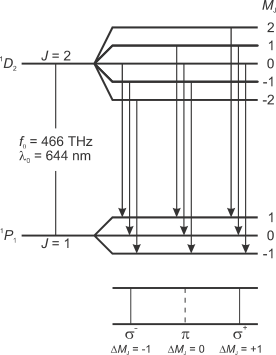
\includegraphics[width=.4\linewidth]{Niveauaufspaltung_Cd.png}
    \caption[Niveauaufspaltung des$5^1D_2 \rightarrow 5^1P_1$-Übergangs bei Cd]{Niveauaufspaltung des $5^1D_2 \rightarrow 5^1P_1$-Übergangs beim normalen \texttt{Zeemann}-Effekt an Cadmium~\cite{LD}}\label{fig:cd_niveaus}
\end{figure}
%--
\begin{figure}[!ht]
    \centering
    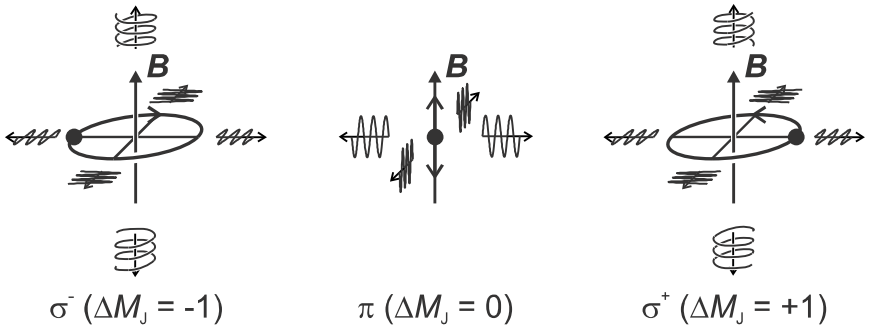
\includegraphics[width=.55\linewidth]{Dipolstrahlung_Verteilung.PNG}
    \caption[Winkelverteilung der elektischen Dipolstrahlung]{Winkelverteilung der elektischen Dipolstrahlung; $\Delta M_J$ -- Drehimpulsrichtung der emittierten Photonen~\cite{LD}}\label{fig:polarisation} % chktex 8
\end{figure}
%
% -----
%
%\clearpage
\section{Aufbau}
Zur Untersuchung des \texttt{Zeemann}-Effekts wird eine Cadmiumlampe verwendet, deren Emissionsspektrum die relevante rote Spektrallinie bei $\lambda = 644 \, \mathrm{nm}$ enthält. Die Lampe befindet sich zwischen den Polschuhen eines Elektromagneten, dessen homogenes Magnetfeld durch ein Hochstromnetzgerät erzeugt und über eine Hall-Sonde kallibriert wird. Die optische Strahlführung umfasst folgende Komponenten zu Erzeugung eines Interferenzbildes (siehe \cref{fig:aufbau_zeemann}):
%--
\begin{itemize}
    \item Eine \textbf{Kondensorlinse} (Brennweite $f = \SI{150}{\milli\meter}$ erzeugt eine parallele Beleuchtung).
    \item Ein \textbf{Fabry-Pérot-Etalon} mit einem Plattenabstand von $d = \SI{4}{\milli\meter}$, einem Brechungsindex $n = 1.457$ und einem Reflexionsgrad von $R = 0.85$.
    \item Eine Abbildungslinse (ebenfalls $f = \SI{150}{\milli\meter}$) bildet die Interferenzringe ab.
    \item Ein \textbf{Interferenzfilter} mit einer Mittelwellenlänge von $\lambda = \SI{643,8\pm 2,0}{\nano\meter}$ selektiert die zu untersuchende Spektrallinie.
    \item Zur Analyse der Polarisation werden ein Polarisationsfilter und eine Viertelwellenlängeplatte verwendet.
\end{itemize}
%--
\begin{figure}[ht]
    \centering
    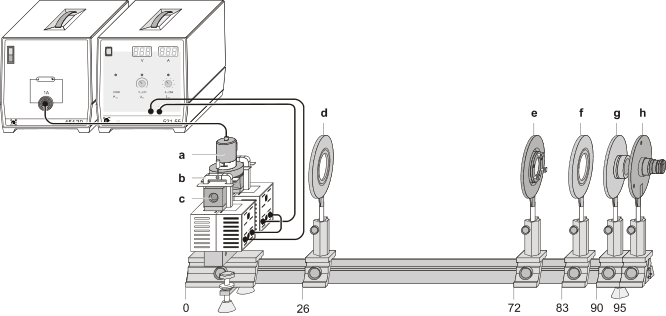
\includegraphics[width=.7\linewidth]{ZeemanAufbau.png}
    \caption[Aufbau der Versuchsanordnung zum Zeemann-Effekt]{Versuchsaufbau zur Messung des \texttt{Zeemann}-Effekts mit (a) Cadmiumlampe, (b) Klammern, (c) Polschuhe, (d) / (f) Sammellinsen, (e) Fabry-Pérot-Etalon, (g) Interferenzfilter und (h) Okular mit Strichskala~\cite{LD}.}\label{fig:aufbau_zeemann}
\end{figure}
%--
Die Beobachtung erfolgt zunächst mit einem Okular. Für die quantitative Auswertung wird das Okular dann durch eine CCD-Kamera ersetzt, welche das Intensitätsprofil der Interferenzringe entlang einer Linie in das Messprogramm überträgt.
\vspace{0.3cm}\\
Das \texttt{Fabry-Pérot}-Etalon (\cref{fig:fabry_perot}) ist ein Interferometer, das zur hochauflösung spektraler Aufspaltung genutzt wird. Es besteht aus zwei planparallelen, hochreflektierenden Glasplatten mit einem festen Abstand $d$ zueinander. Licht, dass in einem bestimmten Winkel $\alpha$ in das Etalon eintritt, wird an den beiden Platten mehrfach hin- und herreflektiert, sodass durch Interferenz bestimmte Wellenlängen konstruktiv verstärkt und andere ausgelöscht werden.
%--
\begin{figure}[ht]
    \centering
    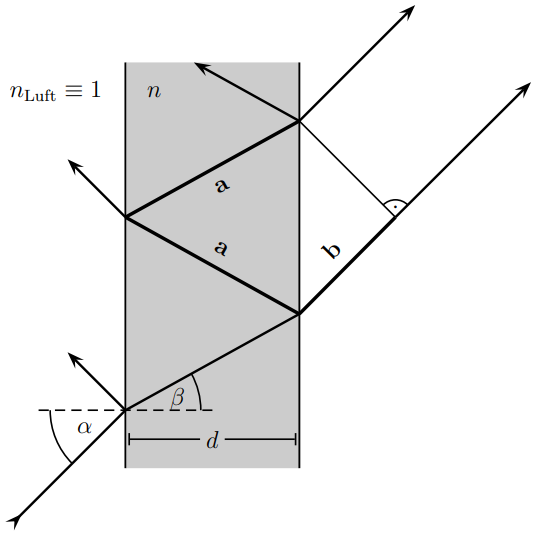
\includegraphics[width=.4\linewidth]{Fabry_Perot.PNG}
    \caption[Fabry-Pérot-Etalon]{Intensität der Interferenzringe in Abhängigkeit von der Wellenlänge~\cite{LD}.}\label{fig:fabry_perot}
\end{figure}
%--

\noindent Die Bedingung für konstruktive Interferenz ergibt sich aus dem optischen Wegunterschied zwischen den reflektierten Teilstrahlen:
%--
\begin{equation}
    2nd \cos(\alpha) = m \lambda
\end{equation}
%--
wobei $n$ der Brechungsindex des Mediums zwischen den Platten, $d$ der Abstand der Platten, $m \in \mathbb{Z}$ die Interferenzrdnung und $\lambda$ die Wellenlänge des Lichts ist.\\
Die resultierende Intensitätsverteilung zeigt sich in Form konzentischer Ringe (Interferenzringe), die bei Verwendung eines monochromatischen Lichtfilters einer bestimmten Spektrallinie zugeordnet werden können.\\
Die Finesse $\mathcal{F}$ des Etalons beschreibt die Güte der Interferenz und ist definiert als das Verhältnis der Wellenlängenabstände $\Delta \lambda$ der benachbarten Maxima zur Breite $\Delta \lambda_0$ des zentralen Maximums:
%--
\begin{equation}
    \mathcal{F} = \frac{\Delta \lambda}{\Delta \lambda_0} = \frac{\pi\sqrt{R}}{1-R}
\end{equation}
%--
Die Finesse  ist ein Maß für die Anzahl der Interferenzmaxima, die innerhalb einer bestimmten Wellenlängenbreite auftreten können.\\
Die Auflösung $A$ des Etalons ist definiert als das Verhältnis der Wellenlängen $\lambda$ zur Breite $\Delta \lambda$ der Maxima:
%--
\begin{equation}
    A = \frac{\lambda}{\Delta \lambda}
\end{equation}
%--
Die Auflösung ist ein Maß dafür, wie gut das Etalon in der Lage ist, benachbarte Spektrallinien zu trennen.\\
%
%--
%
\section{Beobachtung der Aufspaltung}
%
%--
%
\subsection{Justage}
Nachdem die Lampe für etwa 2 Minuten warm gelaufen ist, wird der optische Aufbau mit Hilfe des Okulars justiert, um ein symmetrisches und zentriertes Interferenzmuster zu erhalten.\\
Dafür wird zunächst das Okular scharf auf die Strichskala eingestellt. Die Cadmiumlampe wird so positioniert, dass die Lichtquelle möglichst mittig im Magnetfeld liegt. Die Kondensorlinse wurde justiert, um eine parallele Ausleuchtung des Etalons zu erreichen.\\
Die Position der zweiten Linse sowie des Beobachtungspfades (jetzt Okular später CCD-Kamera) werden so eingestellt, dass das durch das Fabry-Pérot-Etalon erzeugte Ringsystem mittig und scharf abgebildet wird.\\
Durch leichtes Kippen des Etalons kann das Zentrum des Ringsystems auf die Strichskala eingestellt werden.
\vspace{0.3cm}\\
Um longitudinale und transversale Konfigurationen zu untersuchen wird die Halterung der Spulen zusammen mit der Cd-Lampe um $90^{\circ}$ gedreht (\cref{fig:aufbau_zeemann_above}).\\
%--
\begin{figure}[H]
    \centering
    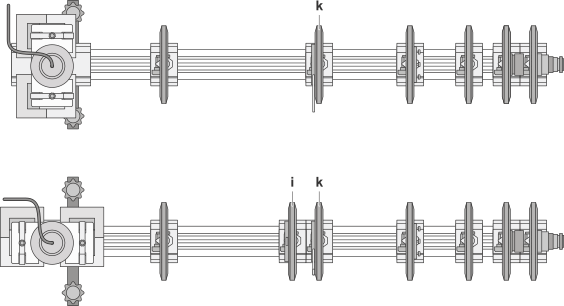
\includegraphics[width=.6\linewidth]{ZeemanAufbaufromAbove.png}
    \caption[Longitudinale und Transversale Konfiguration Zeemann-Effekt]{Aufbau zur Messung in transversaler Konfiguration (oben) und longitudinaler Konfiguration (unten) von oben betrachtet mit (i) Viertel-Wellenlängen-Platte und (k) Polarisationsfilter~\cite{LD}.}\label{fig:aufbau_zeemann_above}
\end{figure}
%--
\noindent Zur Beobachtung der jeweiligen Komponenten werden die Polarisationsfilter und die Viertelwellenlängenplatte in den Strahlengang eingebaut.\\
%
%--
%
\subsection{Transversale Konfiguration}
%--
\begin{figure}[ht]
    \begin{center}
        \subcaptionbox{\texttt{Zeemann}-Aufspaltung in transversaler Konfiguration (A) ohne Magnetfeld, (B) mit Magnetfeld, (C) mit Polarisationsfilter auf $0^{\circ}$ und (D) mit Polarisationsfilter auf $90^{\circ}$. Für das Magnetfeld wurde der Strom jeweils auf $\SI{6,9}{\ampere}$ eingestellt}{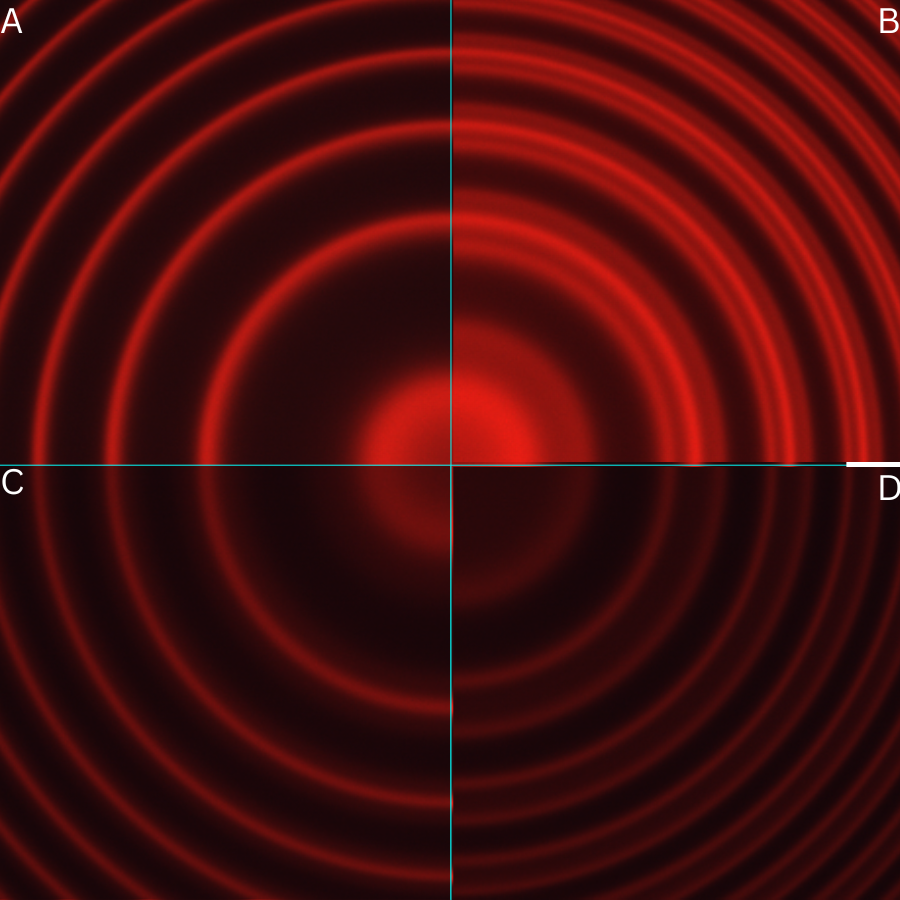
\includegraphics[width=0.49\textwidth]{Transversal.png}}\label{fig:trans_all}
        \subcaptionbox{Einstellung des Stroms auf $\SI{4,7}{\ampere}$ bis die aufgespalteten Linien ohne Filter gerade unterschieden werden können}{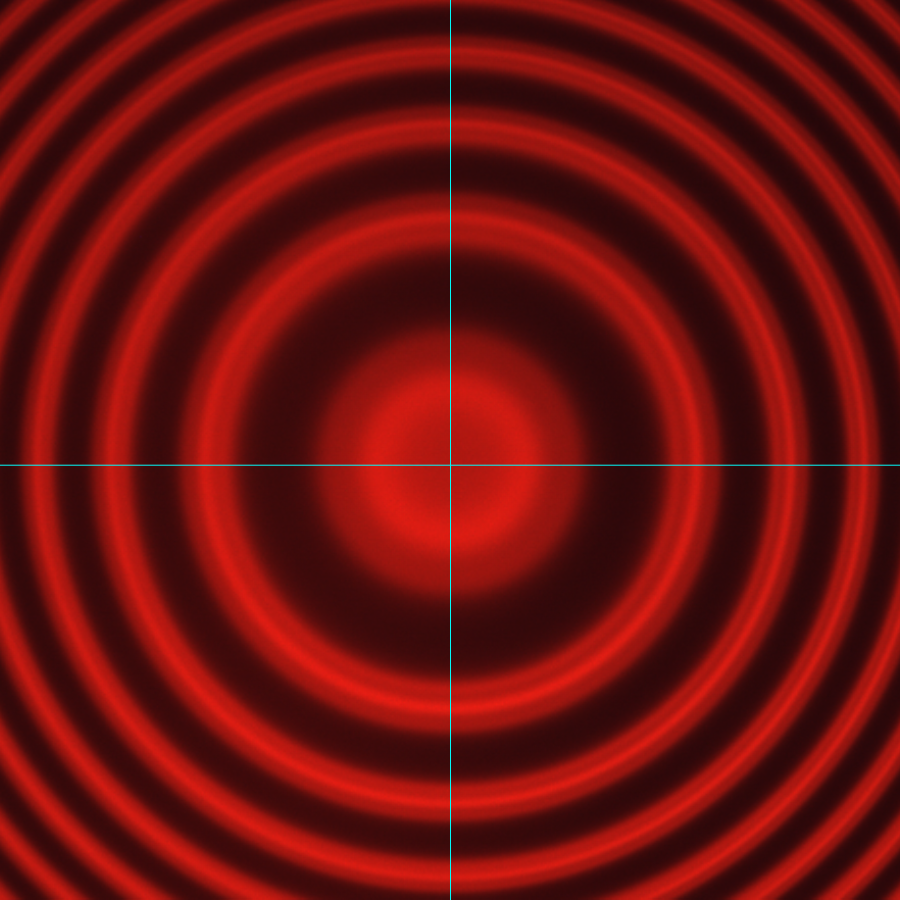
\includegraphics[width=0.49\textwidth]{Trans_Strom.png}}\label{fig:trans_strom}
    \end{center}
\end{figure}
%--
\clearpage
\noindent Bei Ausgeschaltetem Magnetfeld (\cref{fig:trans_all} (A)) sind die konzentrischen Interferenzringe durch Mehrfachinterferenz von kohärentem Licht im Etalon sichtbar. Die verwendetete Cd-Lampe emmitiert spektrale Linien, unter anderem bei einer Wellenlänge von $\lambda = \SI{643,8}{\nano\meter}$, die einem elektronischen Übergang vom angeregten Zustand $5^1D_2$ in den Grundzustand $5^1P_1$ entspricht. Um sicherzustellen, dass ausschließlich diese Übergangslinie beobachtet wird, wird durch den Interferenzfilter eine Durchlassbreite von $\pm \SI{2}{\nano\meter}$ ausgewählt.
\vspace{0.2cm}\\
Der Magnetstrom wird auf $\SI{6,9}{\ampere}$ eingestellt, sodass die Aufspaltung der Spektrallinie sichtbar wird (\cref{fig:trans_all} (B)). Der mittlere Ring ist dabei am stärksten ausgeprägt und entspricht der $\pi$-Komponente ($\Delta M_J=0$), während die äußeren Ringe innen schwächer sind und den $\sigma^\pm$-Komponenten ($\Delta M_J=\pm 1$) entsprechen.\\ 
Die $\sigma$-Komponenten werden über ihre radiale Verschiebung im Interferenzbild identifiziert: Die Linie mit geringerer Wellenlänge ($\sigma^+$) ist nach außen verschoben, die Linie mit größerer Wellenlänge ($\sigma^-$) nach innen.\\
Die intensität der Komponenten variiert im Verlauf der Messung, insbesondere im Vergleich zum Bild ohne Magnetfeld.
\vspace{0.2cm}\\
\noindent Bei Verwendung des Polarisationsfilters auf $0^{\circ}$ (\cref{fig:trans_all} (C)) zwischen Kondensonrlinse und Etalon werden die $\sigma^\pm$-Komponenten aufgrund ihrer Polarisationsrichtung herausgefiltert.
\vspace{0.2cm}\\
\noindent Wird der Polarisationsfilters nun auf $90^{\circ}$ eingestellt (\cref{fig:trans_all} (D)), wird die $\pi$-Komponente herausgefiltert, sodass nur die $\sigma^\pm$-Komponenten sichtbar sind.
%
%--
%
\subsection{Longitudinale Konfiguration}
%--
\begin{figure}[ht]
    \begin{center}
        \subcaptionbox{\texttt{Zeemann}-Aufspaltung in longitudinaler Konfiguration (A) ohne Magnetfeld, (B) mit Magnetfeld, (C) mit Viertel-Wellenlänge-Platte auf $0^{\circ}$ und Polarisationsfilter auf $-45^{\circ}$ und (D) mit Viertel-Wellenlänge-Platte auf $0^{\circ}$ und mit Polarisationsfilter auf $+45^{\circ}$. Für das Magnetfeld wurde der Strom jeweils auf $\SI{2,5}{\ampere}$ eingestellt}{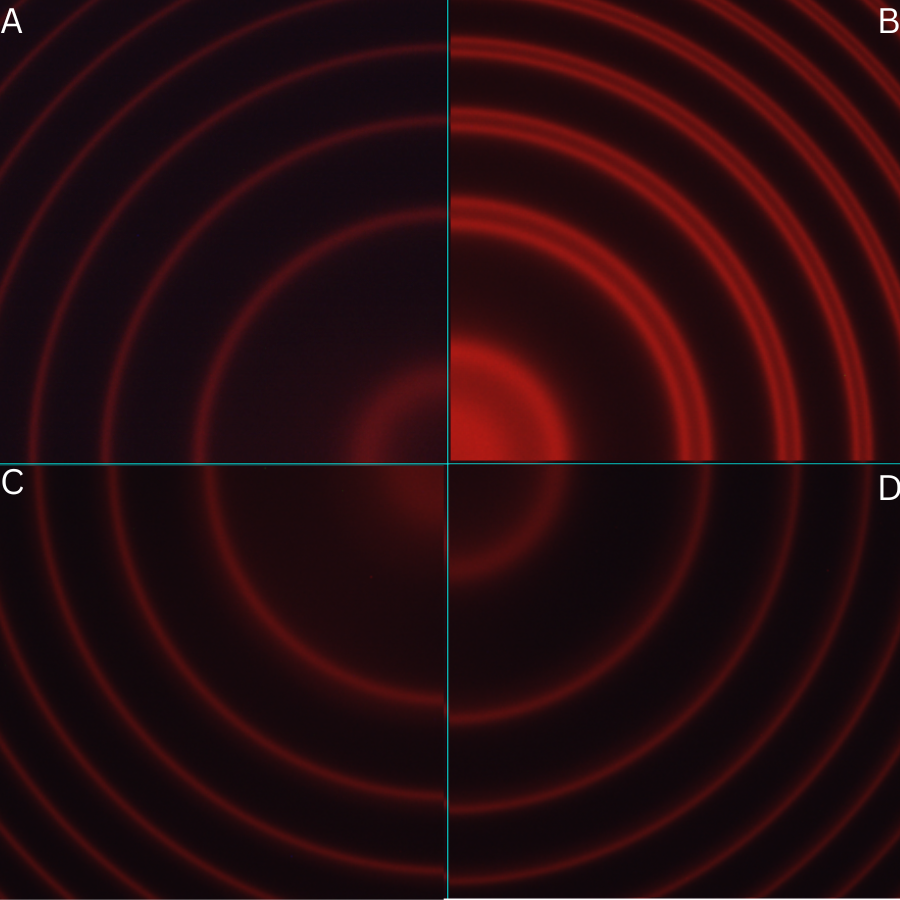
\includegraphics[width=0.49\textwidth]{Longitudinal.png}}\label{fig:long_all}
        \subcaptionbox{Einstellung des Stroms auf $\SI{1,7}{\ampere}$ bis die aufgespalteten Linien ohne Filter gerade unterschieden werden können}{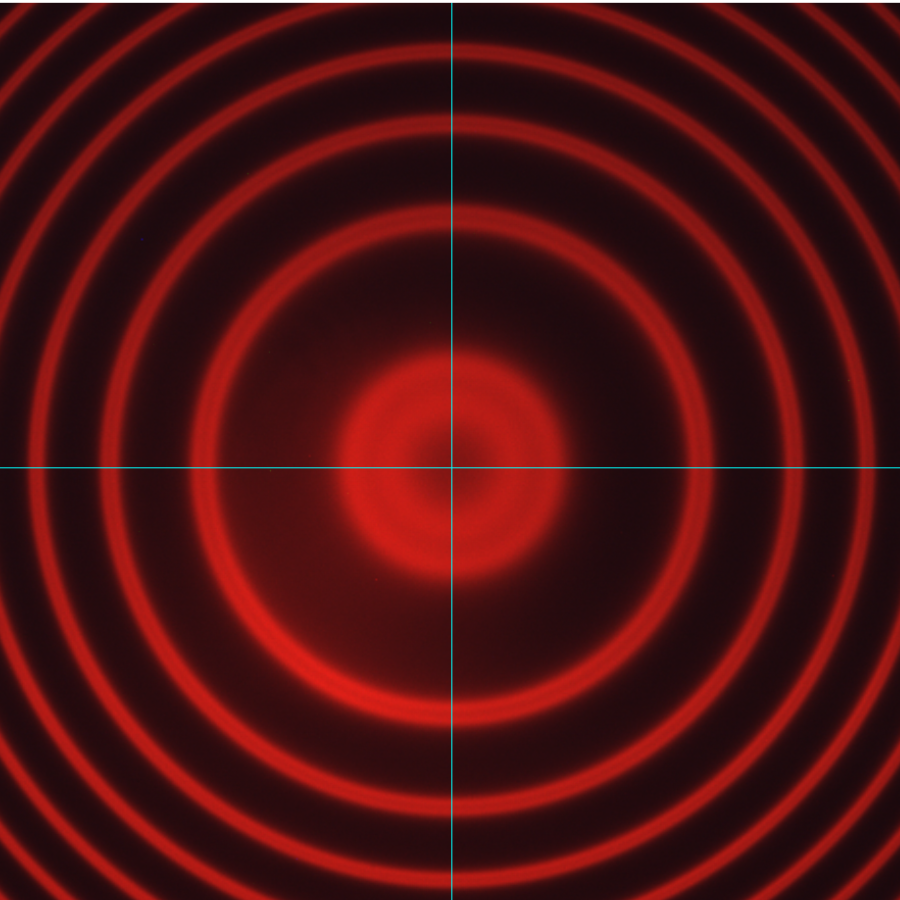
\includegraphics[width=0.49\textwidth]{Long_Strom.png}}\label{fig:long_strom}
    \end{center}
\end{figure}
\chapter{Franck-Hertz-Versuch}

\section{Section}
% ----------------------------------------------------------------------------------
% ----------------------------------------------------------------------------------
\
\begin{figure}[H]
    \centering
    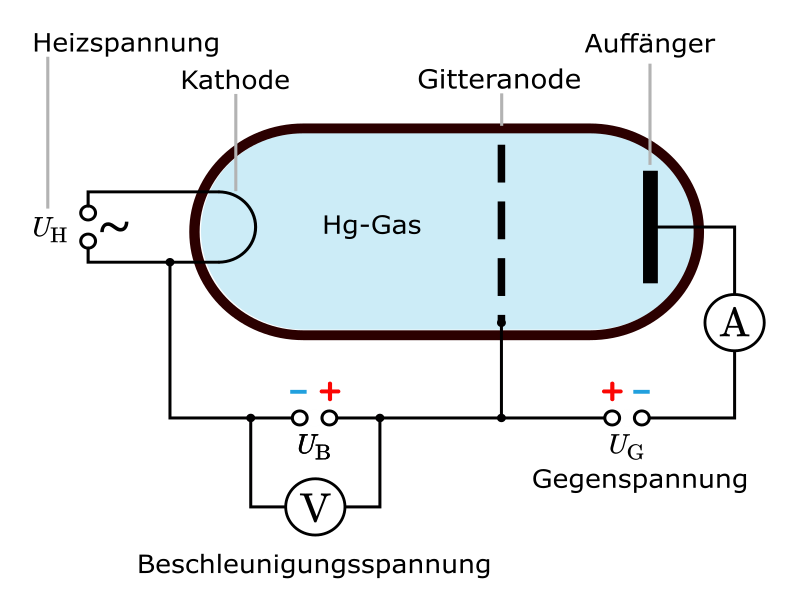
\includegraphics[width=0.5\textwidth]{FranckHertzAufbau.png}
    \caption{Franck-Hertz-Schaltung}
    \label{fig:FrankHertzSchaltung}    
\end{figure}

\subsection{Subsection}

\subsubsection{Subsubsection}

%\begin{table}[h!]
%    \centering
%    \begin{tabular}{
%        l|
%        S[table-format=2.3(3)]
%        S[table-format=1.3(4)]
%        S[table-format=2.3(4)]
%        S[table-format=1.3(4)]
%    }
%    \toprule
%    \multicolumn{1}{l|}{} & 
%    \multicolumn{1}{c}{$a$ [T]} & 
%    \multicolumn{1}{c}{$b$ [T/A]} & 
%    \multicolumn{1}{c}{$c$ [T/A$^2$]} & 
%    \multicolumn{1}{c}{$d$ [T/A$^3$]} \\
%    \midrule
%    Kalibrierung 1 & -0.298 \pm 0.094 & 2.090 \pm 1.265 & 60.782 \pm 4.208 & 0.927 \pm 2.698 \\
%    Kalibrierung 2 & -0.297 \pm 0.102 & 1.620 \pm 1.349 & 65.446 \pm 4.362 & 0.099 \pm 2.735 \\
%    \midrule
%    Gesamtanpassung & -0.297 \pm 0.098 & 1.855 \pm 1.308 & 63.114 \pm 4.286 & 0.513 \pm 2.716 \\
%    \bottomrule
%    \end{tabular}
%    \caption{Fitparameter der Magnetfeld-Kalibrierungen}
%    \label{tab:kalibrierung}
%\end{table}

%\begin{table}[h!]
%    \centering
%    \begin{tabular}{
%        l|
%        S[table-format=2.3(3)]
%        S[table-format=1.3(4)]
%        S[table-format=2.3(4)]
%        S[table-format=1.3(4)]
%    }
%    \toprule
%    \multicolumn{1}{l|}{} & 
%    \multicolumn{1}{c}{$a$ [T]} & 
%    \multicolumn{1}{c}{$b$ [T/A]} & 
%    \multicolumn{1}{c}{$c$ [T/A$^2$]} & 
%    \multicolumn{1}{c}{$d$ [T/A$^3$]} \\
%    \midrule
%    Gesamtanpassung & -0.297 \pm 0.098 & 1.855 \pm 1.308 & 63.114 \pm 4.286 & 0.513 \pm 2.716 \\
%    \bottomrule
%    \end{tabular}
%    \caption{Fitparameter der Gesamtanpassung der Magnetfeld-Kalibrierungen}
%    \label{tab:kalibrierung2}
%\end{table}   

%\begin{table}[H]
%    \centering
%    \footnotesize
%    \begin{tabular}{c *{5}{c}}
%        \toprule
%        Parameter & {1} & {2} & {3} & {4} & {5} \\
%        \midrule
%        $\chi_\text{red}^2$ & 1.34      & 1.68              & 1.11          & 0.72              & 0.83 \\
%        $a$         & 2.85 (0.92)       & -8.53 (9.96)      & 9.92 (---)    & 0.043 (1.26)      & 10.96 (2.10) \\
%        $b$         & 8.15 (1.43)       & 26.12 (15.02)     & -1.57 (---)   & 17.05 (1.94)      & -0.96 (3.53) \\
%        $A_1$       & 0.046 (0.015)     & 0.008 (0.0043)    & 7.1e-7 (---)  & 0.803 (0.077)     & 1.336 (0.185) \\
%        $\sigma_1$  & 0.015 (0.0030)    & 0.0049 (0.0025)   & 0.045 (---)   & 0.024 (0.0013)    & 0.031 (0.0024) \\
%        $\mu_1$     & 1.559 (0.0029)    & 1.537 (0.0022)    & 1.547 (---)   & 1.573 (0.0022)    & 1.569 (0.0030) \\
%        $A_2$       & 3.201 (0.228)     & 4.301 (0.194)     & 4.672 (---)   & 0.831 (0.191)     & 1.835 (0.228) \\
%        $\mu_2$     & 1.644 (0.0023)    & 1.649 (0.0009)    & 1.649 (---)   & 1.625 (0.0018)    & 1.635 (0.0014) \\
%        $\sigma_2$  & 0.0349 (0.0012)   & 0.0453 (0.0008)   & 0.0533 (---)  & 0.0229 (0.0021)   & 0.0279 (0.0017) \\
%        $A_3$       & 0.488 (0.243)     & 0.575 (0.376)     & 0.146 (---)   & 3.705 (0.235)     & 2.473 (0.194) \\
%        $\mu_3$     & 1.711 (0.013)     & 1.761 (0.0087)    & 1.725 (---)   & 1.682 (0.0027)    & 1.709 (0.0022) \\
%        $\sigma_3$  & 0.0340 (0.0062)   & 0.0426 (0.0100)   & 0.0346 (---)  & 0.0502 (0.0020)   & 0.0403 (0.0020) \\
%        \bottomrule
%    \end{tabular}
%    \vspace{1em}
%    \begin{tabular}{c *{5}{c}}
%        \toprule
%        Parameter & {6} & {7} & {8} & {9} & {10} \\
%        \midrule
%        $\chi_\text{red}^2$ & 0.858 & 0.825 & 0.620 & 0.674 & 0.669 \\
%        $a$         & 10.04 (3.07)      & 18.77 (4.66)      & 22.47 (6.25)      & 46.72 (13.07)     & -21.55 (15.45) \\
%        $b$         & 2.92 (4.93)       & -10.10 (8.08)     & -15.89 (10.80)    & -56.16 (23.80)    & 54.46 (22.96) \\
%        $A_1$       & 1.223 (0.128)     & 1.183 (0.195)     & 1.226 (0.234)     & 1.896 (0.566)     & 1.029 (0.194) \\
%        $\sigma_1$  & 0.0293 (0.0017)   & 0.0312 (0.0025)   & 0.0325 (0.0027)   & 0.0387 (0.0043)   & 0.0288 (0.0022) \\
%        $\mu_1$     & 1.560 (0.0015)    & 1.551 (0.0014)    & 1.546 (0.0012)    & 1.541 (0.0019)    & 1.545 (0.0010) \\
%        $A_2$       & 2.263 (0.117)     & 2.608 (0.0833)    & 2.692 (0.105)     & 2.509 (0.207)     & 2.673 (0.259) \\
%        $\mu_2$     & 1.639 (0.00087)   & 1.641 (0.00074)   & 1.642 (0.00057)   & 1.643 (0.00091)   & 1.642 (0.00051) \\
%        $\sigma_2$  & 0.0311 (0.0014)   & 0.0364 (0.0014)   & 0.0375 (0.0010)   & 0.0351 (0.0007)   & 0.0363 (0.0008) \\
%        $A_3$       & 2.010 (0.188)     & 1.542 (0.155)     & 1.578 (0.189)     & 1.202 (0.151)     & 2.541 (0.716) \\
%        $\mu_3$     & 1.727 (0.0015)    & 1.739 (0.0010)    & 1.746 (0.00086)   & 1.747 (0.00078)   & 1.758 (0.0018) \\
%        $\sigma_3$  & 0.0375 (0.0021)   & 0.0325 (0.0017)   & 0.0331 (0.0018)   & 0.0288 (0.0015)   & 0.0410 (0.0042) \\
%        \bottomrule
%    \end{tabular}
%    \caption[Anpassungsparameter zur Messreihe \textsc{Zeeman}-Effekt]{Anpassungsparameter der Gaußkurven aus der Messreihe zum \textsc{Zeeman}-Effekt. Die dazugehörigen Abbildungen sind \crefrange{subfig:1}{subfig:10} zu finden.}
%    \label{tab:langzeeman-fit}
%\end{table}
%\normalsize
%
\begin{table}[h!]
    \centering
    \begin{tabular}{
        S[table-format=1]
        S[table-format=2.3(3)]
        S[table-format=1.3(4)]
    }
    \toprule
    \multicolumn{1}{c}{Messungs-Nr.} & 
    \multicolumn{1}{c}{Spulenstrom [A]} & 
    \multicolumn{1}{c}{Magn. Flussdichte [T]} \\
    \midrule
    1 & 1.0 \pm 0.015 & 65.18 \pm 1.31 \\
    2 & 2.0 \pm 0.030 & 131.78 \pm 2.64 \\
    3 & 3.0 \pm 0.045 & 198.52 \pm 3.97 \\
    4 & 4.0 \pm 0.060 & 263.61 \pm 5.28 \\
    5 & 5.0 \pm 0.075 & 325.27 \pm 6.51 \\
    6 & 6.0 \pm 0.090 & 381.72 \pm 7.64 \\
    7 & 7.0 \pm 0.105 & 431.18 \pm 8.63 \\
    8 & 8.0 \pm 0.120 & 471.85 \pm 9.44 \\
    9 & 9.0 \pm 0.135 & 501.95 \pm 10.04 \\
    10 & 10.0 \pm 0.150 & 519.70 \pm 10.40 \\
    \bottomrule
    \end{tabular}
    \caption{Fitparameter der Gesamtanpassung der Magnetfeld-Kalibrierungen}
    \label{tab:spulenstroeme}
\end{table}   

\begin{table}[h!]
    \centering
    \begin{tabular}{
        S[table-format=3.3(2)]
        S[table-format=2.3(3)]
        S[table-format=1.3(4)]
    }
    \toprule
    \multicolumn{1}{c}{Magn.Flussdichte [T]} & 
    \multicolumn{1}{c}{$\Delta E_+$[$10^{24}$ J]} & 
    \multicolumn{1}{c}{$\Delta E_+$[$10^{24}$ J]} \\
    \midrule
    381.72 \pm  7.64 & 5.57 \pm 0.22 & 12.12 \pm 0.24 \\  
    431.18 \pm  8.63 & 6.38 \pm 0.21 & 13.60 \pm 0.22 \\ 
    471.85 \pm  9.44 & 6.80 \pm 0.18 & 14.60 \pm 0.19 \\ 
    501.95 \pm 10.04 & 7.22 \pm 0.29 & 15.04 \pm 0.28 \\ 
    519.70 \pm 10.40 & 6.83 \pm 0.16 & 15.54 \pm 0.21 \\ 
    \bottomrule
    \end{tabular}
    \caption{Fitparameter der Gesamtanpassung der Magnetfeld-Kalibrierungen}
    \label{tab:spulenstroeme}
\end{table}  

\begin{table}[h!]
    \centering
    \begin{tabular}{
        S[table-format=3.3(2)]
        S[table-format=2.3(3)]
        S[table-format=1.3(4)]
    }
    \toprule
    \multicolumn{1}{c}{Magn.Flussdichte [T]} & 
    \multicolumn{1}{c}{$\Delta E_+$[$10^{24}$ J]} & 
    \multicolumn{1}{c}{$\Delta E_+$[$10^{24}$ J]} \\
    \midrule

    \bottomrule
    \end{tabular}
    \caption{Fitparameter der Gesamtanpassung der Magnetfeld-Kalibrierungen}
    \label{tab:spulenstroeme}
\end{table}  
\appendix
\printbibliography{}
\listoffigures\addcontentsline{toc}{chapter}{Abbildungsverzeichnis}
\listoftables\addcontentsline{toc}{chapter}{Tabellenverzeichnis}
\chapter{Anhang}
\section{Abbildungen}
\subsection{Zeeman-Effekt}
\begin{figure}[!ht]
    \subcaptionbox{Aufnahmen der Aufspaltung ohne äußeres Magnetfeld}{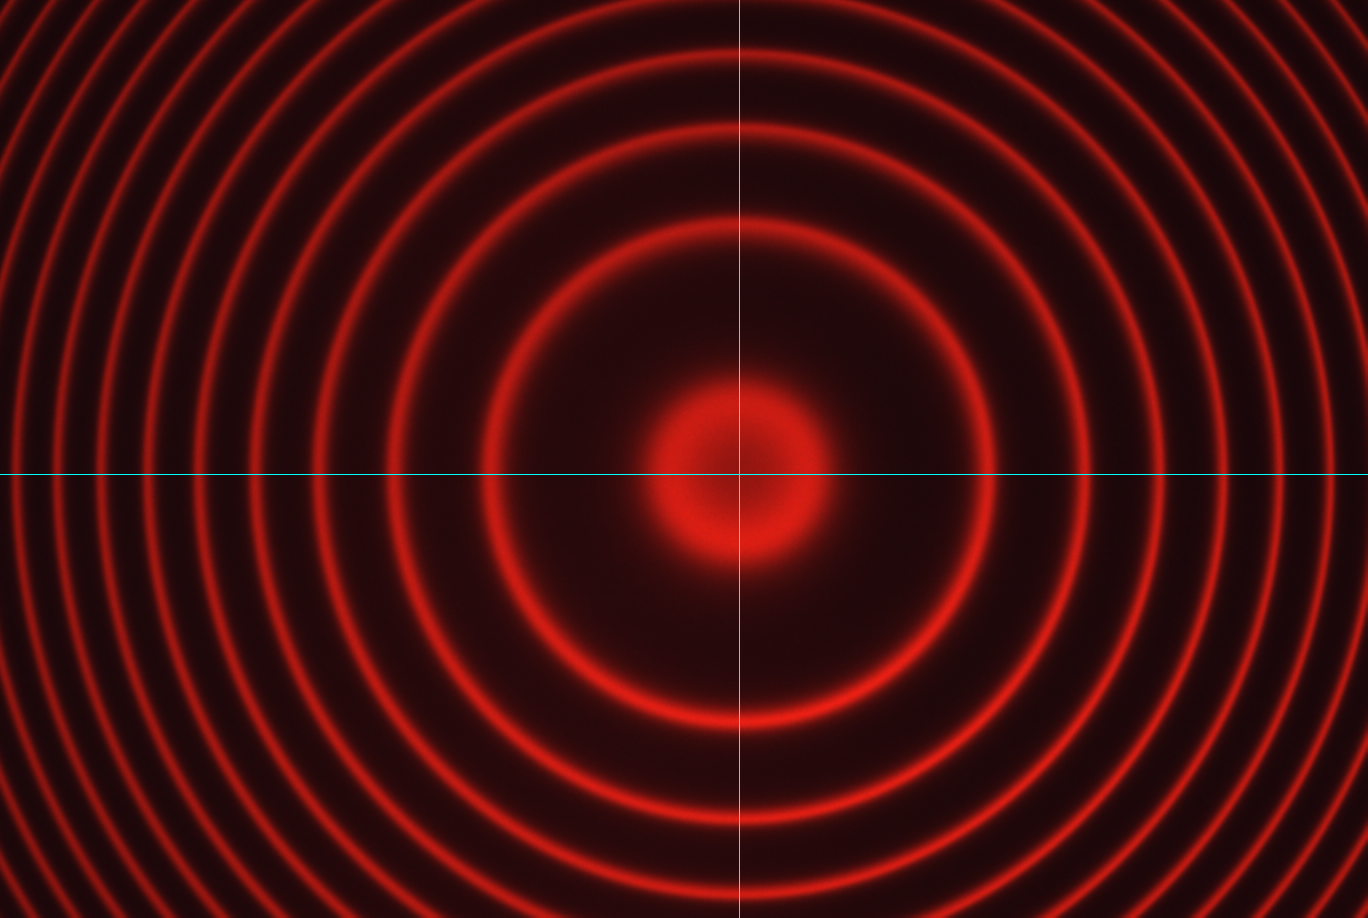
\includegraphics[width=.5\textwidth]{images/ZeemanFoto_001.png}}
    \subcaptionbox{Aufnahmen der Aufspaltung mit äußerem Magnetfeld}{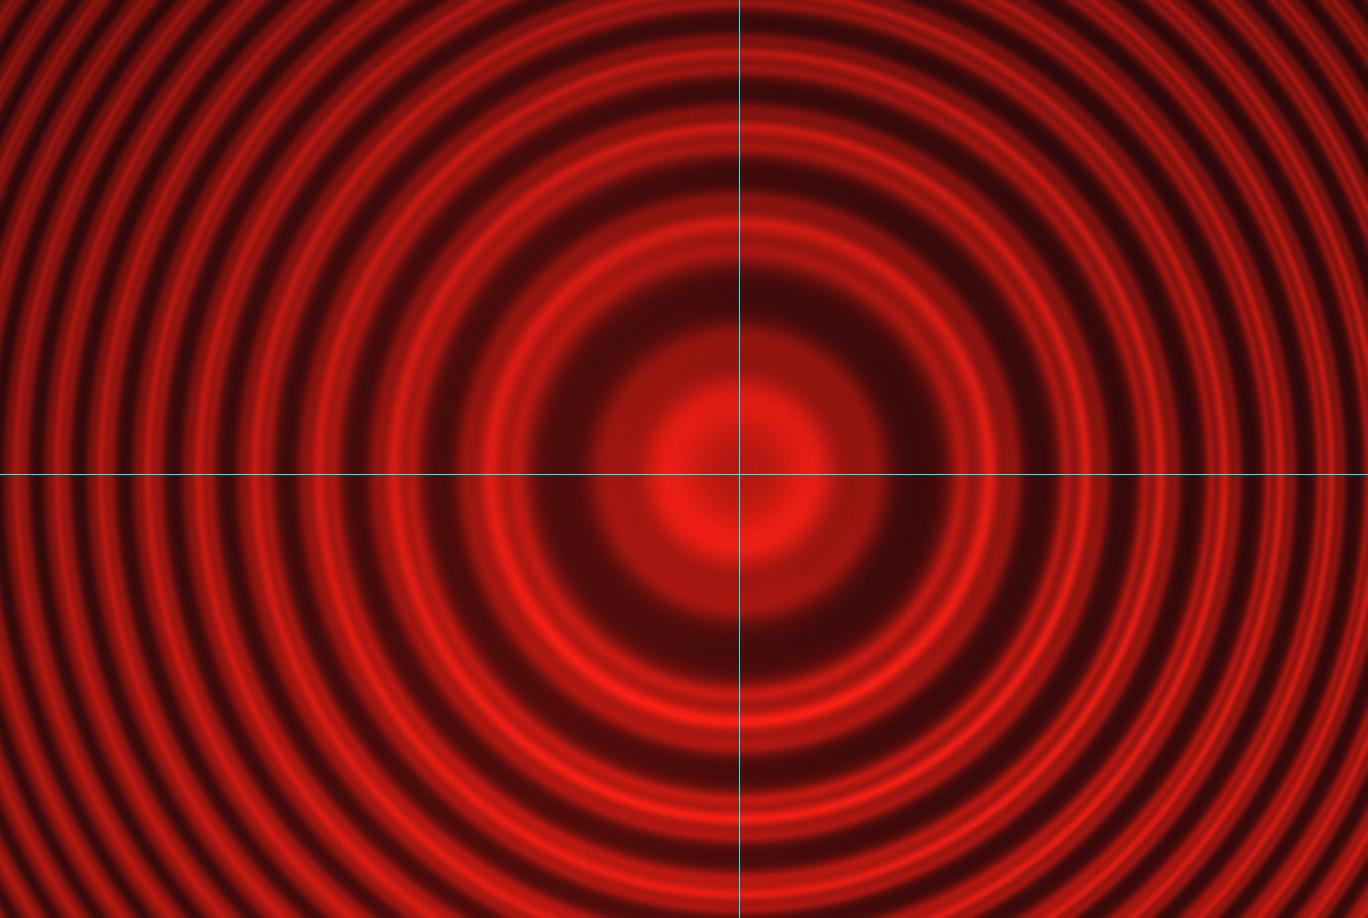
\includegraphics[width=.5\textwidth]{images/ZeemanFoto_002.png}}
    \subcaptionbox{Aufnahmen der Aufspaltung mit äußerem Magnetfeld ($\sigma^{\pm}$-Komponente)}{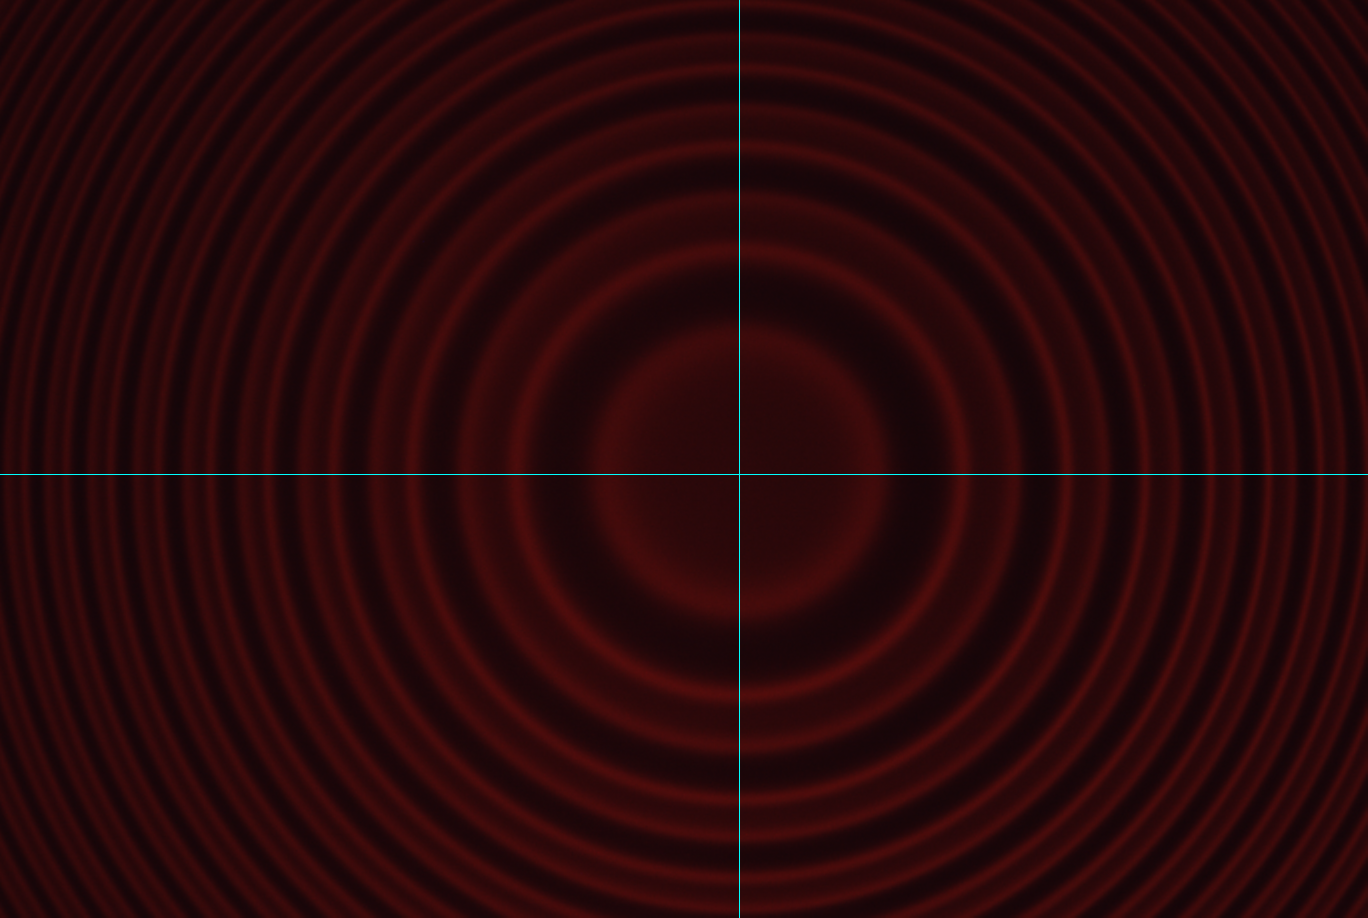
\includegraphics[width=.5\textwidth]{images/ZeemanFoto_003.png}}
    \subcaptionbox{Aufnahmen der Aufspaltung mit äußerem Magnetfeld ($\pi$-Komponente)}{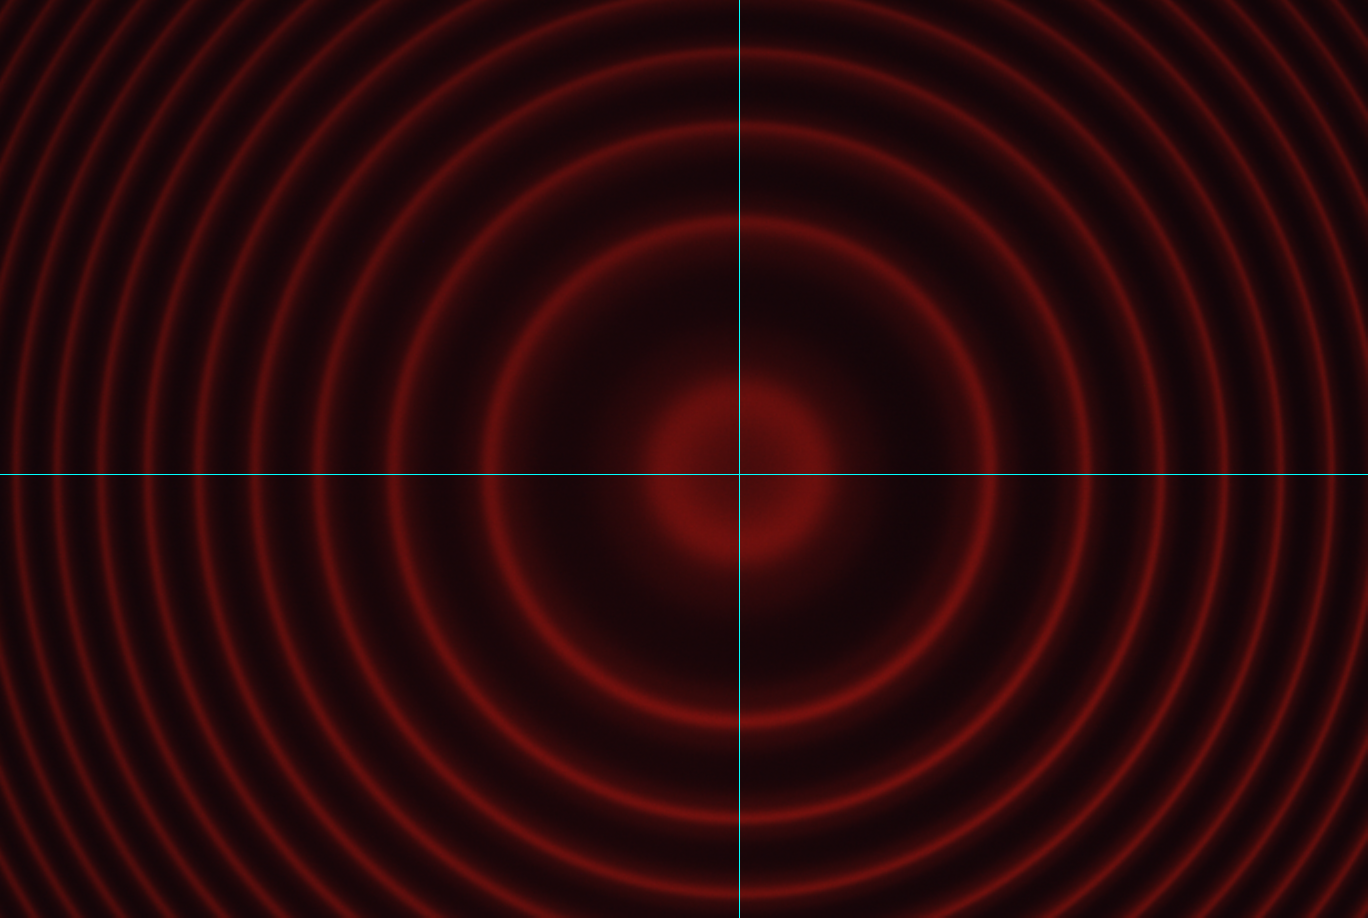
\includegraphics[width=.5\textwidth]{images/ZeemanFoto_004.png}}
    \caption{Aufnahmen in transversaler Konfiguration}
\end{figure}
\begin{figure}[!ht]
    \subcaptionbox{Aufnahmen der Aufspaltung ohne äußeres Magnetfeld}{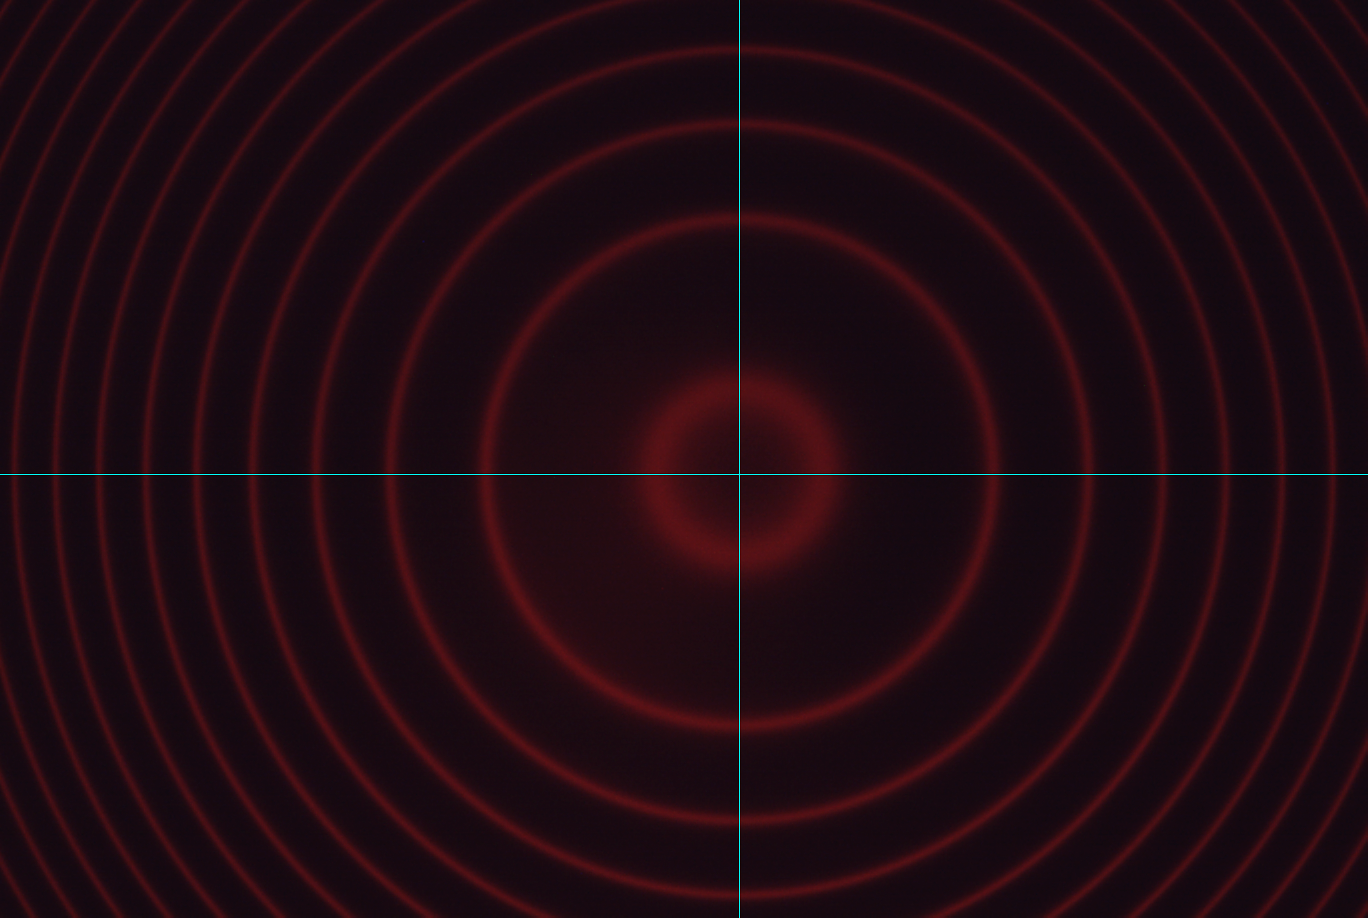
\includegraphics[width=.5\textwidth]{images/ZeemanFoto_008.png}}
    \subcaptionbox{Aufnahmen der Aufspaltung mit äußerem Magnetfeld}{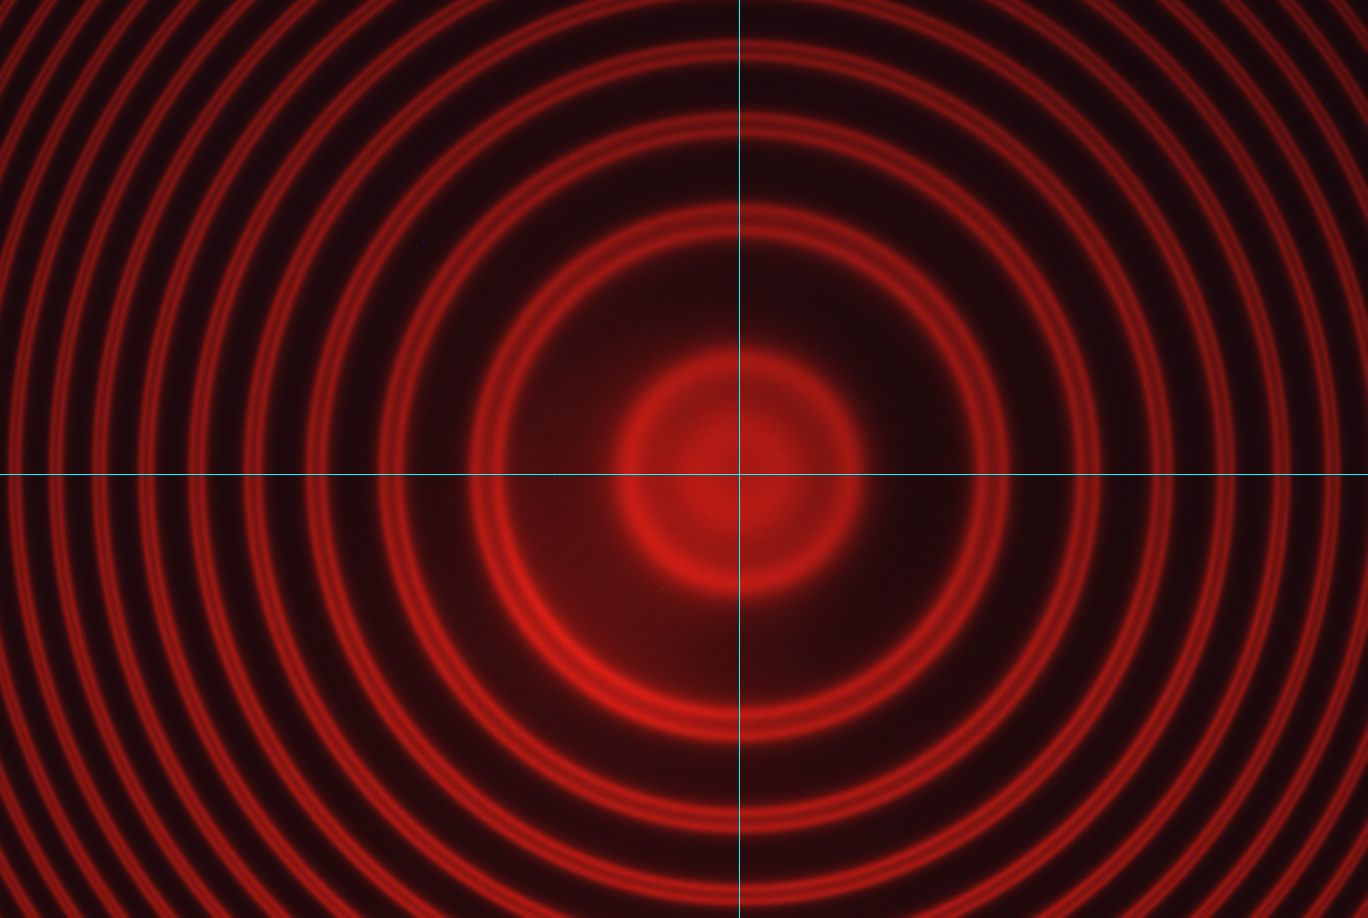
\includegraphics[width=.5\textwidth]{images/ZeemanFoto_009.png}}
    \subcaptionbox{Aufnahmen der Aufspaltung mit äußerem Magnetfeld ($\sigma^{+}$-Komponente)}{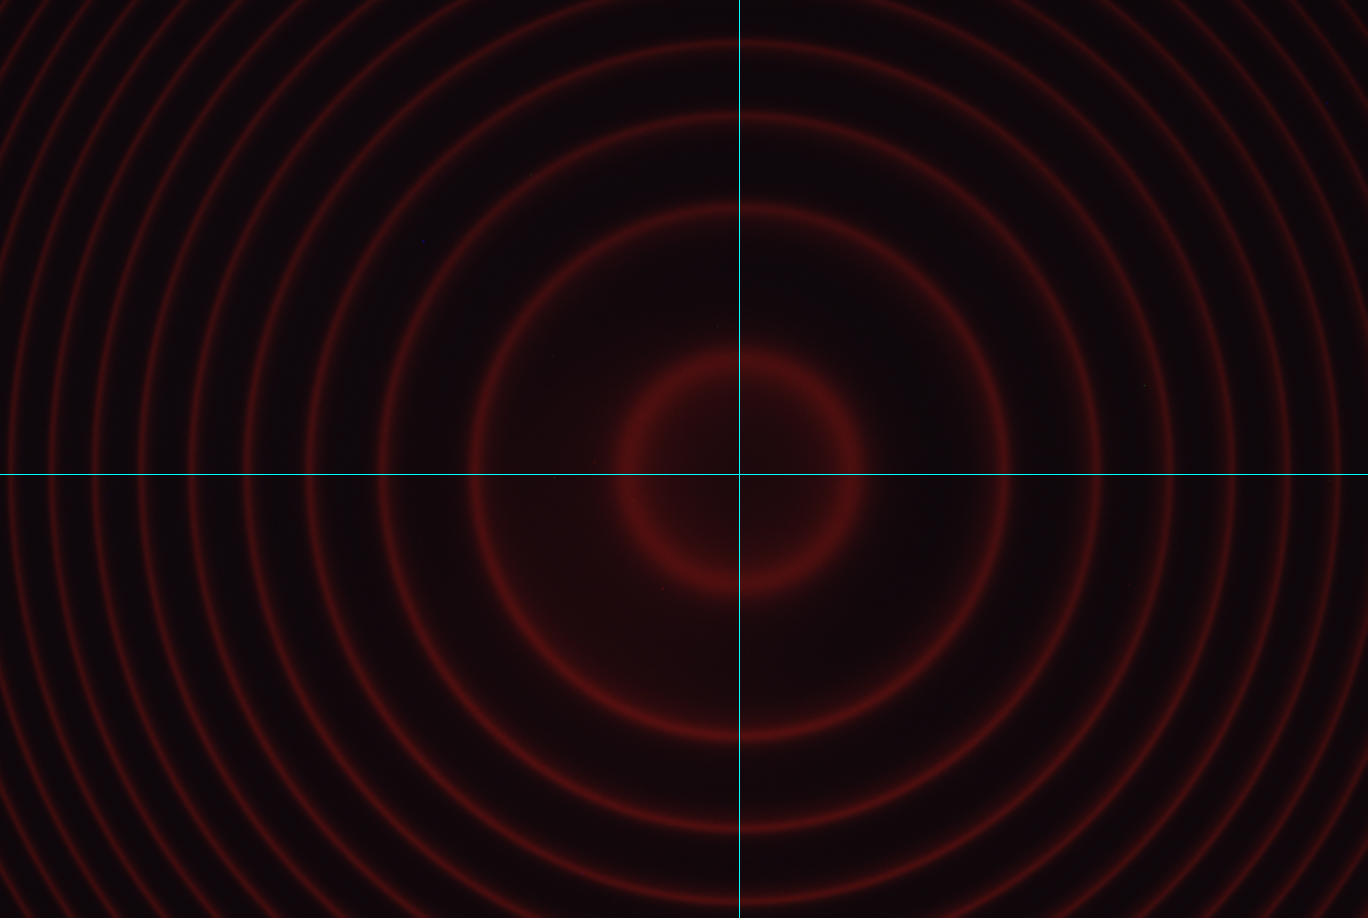
\includegraphics[width=.5\textwidth]{images/ZeemanFoto_010.png}}
    \subcaptionbox{Aufnahmen der Aufspaltung mit äußerem Magnetfeld ($\sigma^-$-Komponente)}{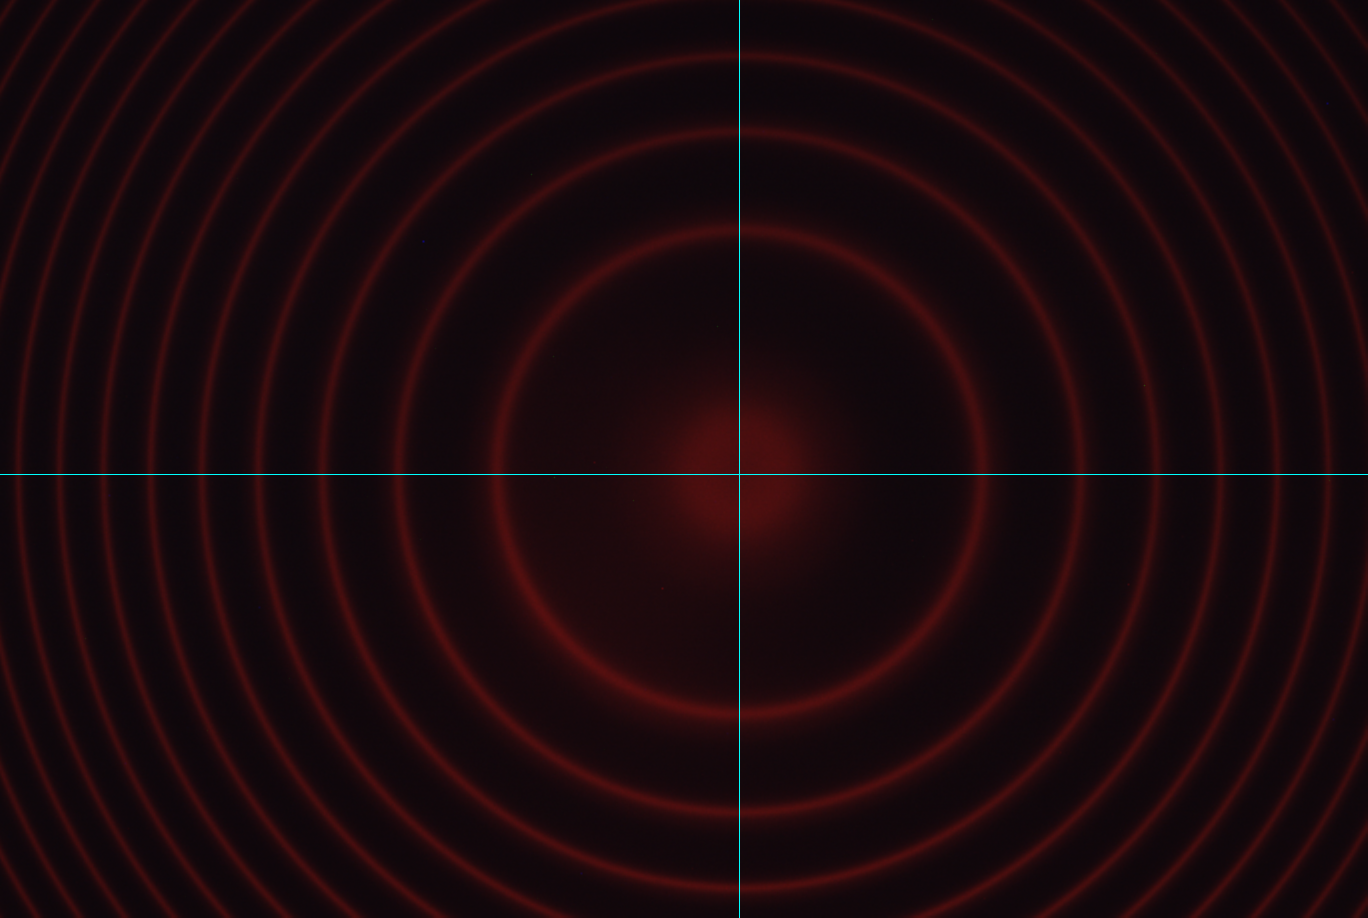
\includegraphics[width=.5\textwidth]{images/ZeemanFoto_011.png}}
    \caption{Aufnahmen in longitudinaler Konfiguration}
\end{figure}
\begin{figure}[!ht]
    \subcaptionbox{Anpassungskurve für $I = \SI{1}{\ampere}$}{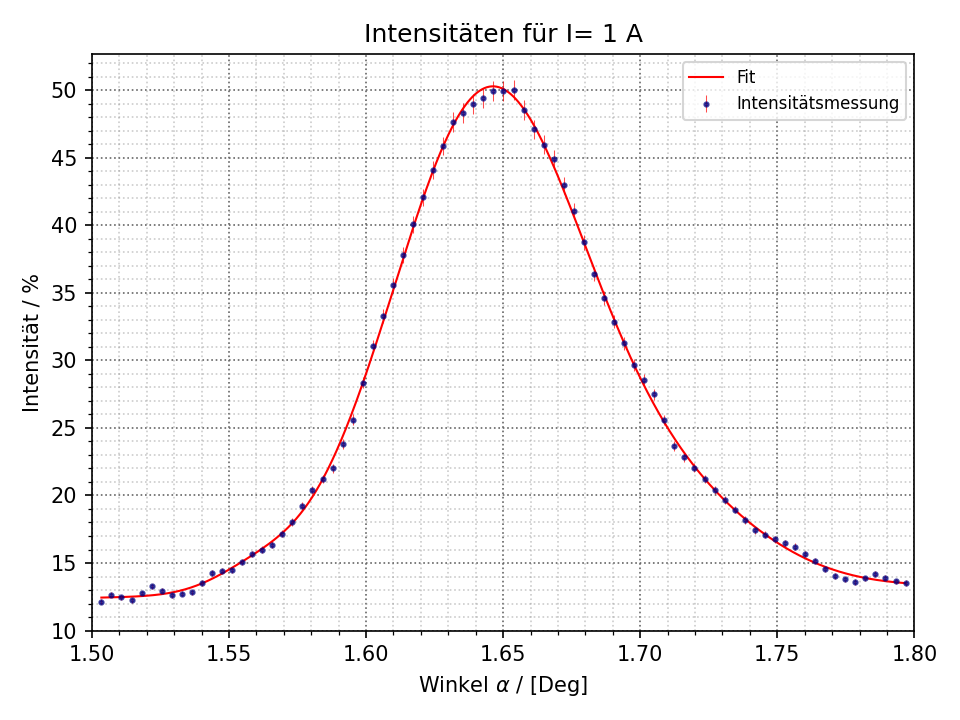
\includegraphics[width=.5\textwidth]{plots/peak_1A}}
    \subcaptionbox{Anpassungskurve für $I = \SI{2}{\ampere}$}{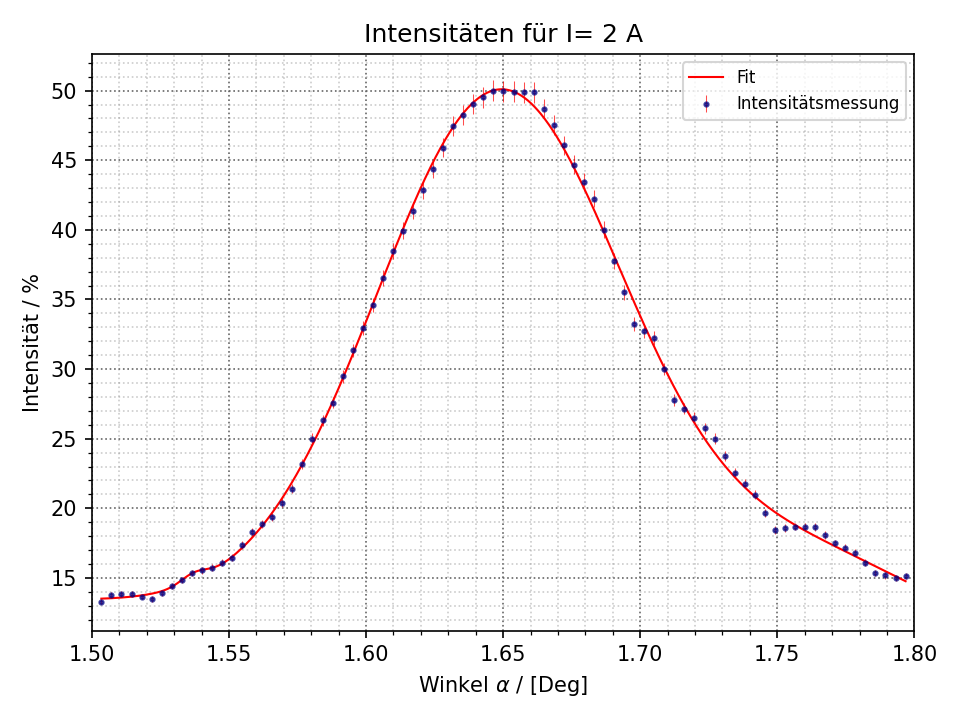
\includegraphics[width=.5\textwidth]{plots/peak_2A}}
    \subcaptionbox{Anpassungskurve für $I = \SI{3}{\ampere}$}{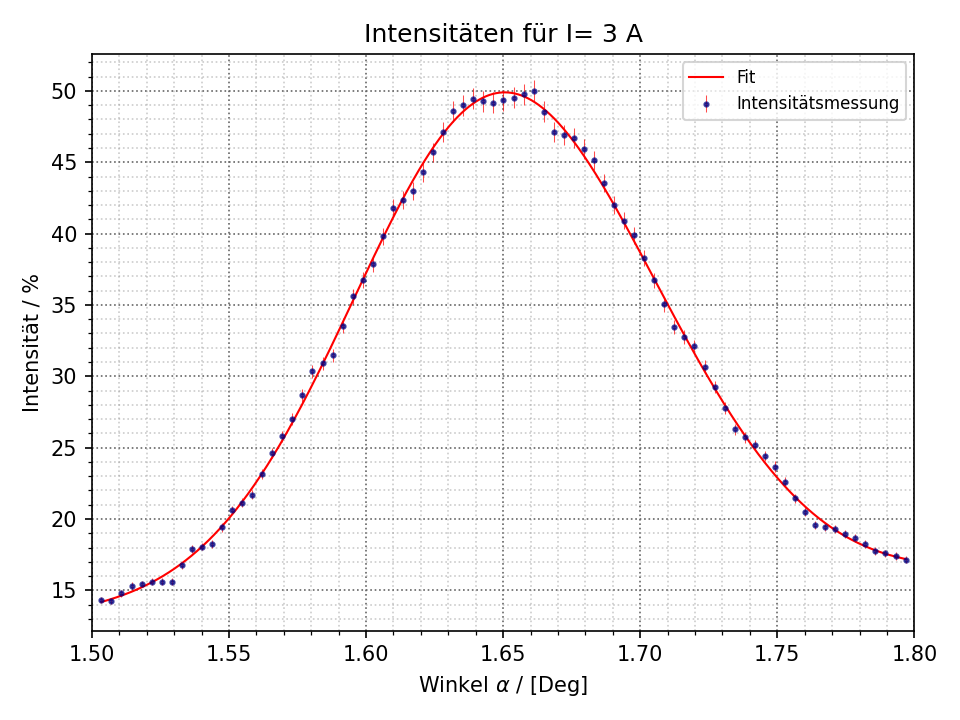
\includegraphics[width=.5\textwidth]{plots/peak_3A}}
    \subcaptionbox{Anpassungskurve für $I = \SI{4}{\ampere}$}{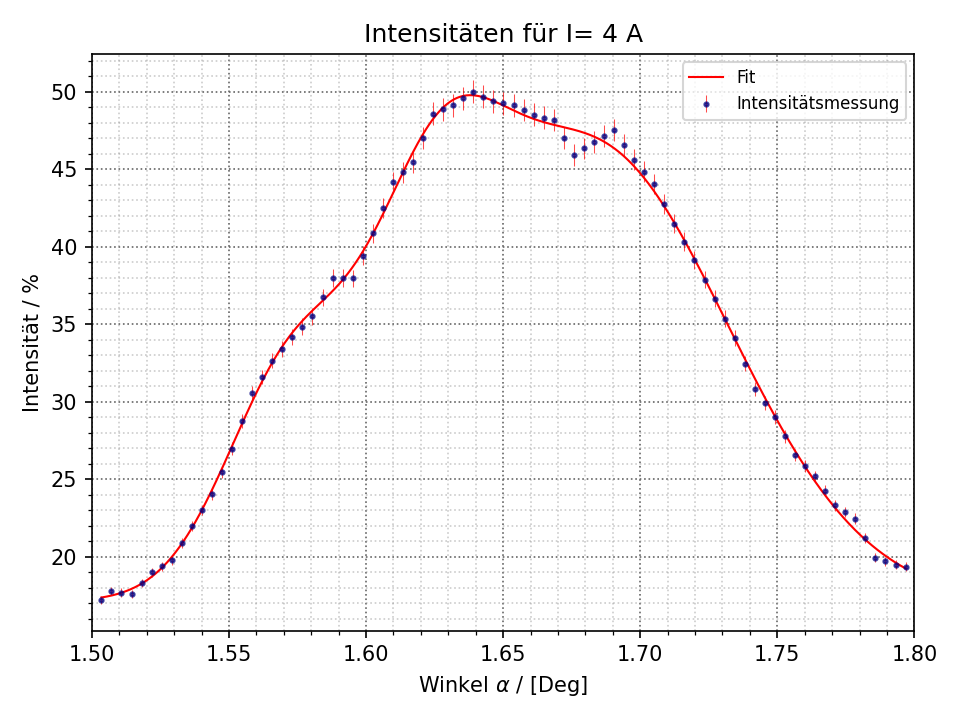
\includegraphics[width=.5\textwidth]{plots/peak_4A}}
    \subcaptionbox{Anpassungskurve für $I = \SI{5}{\ampere}$}{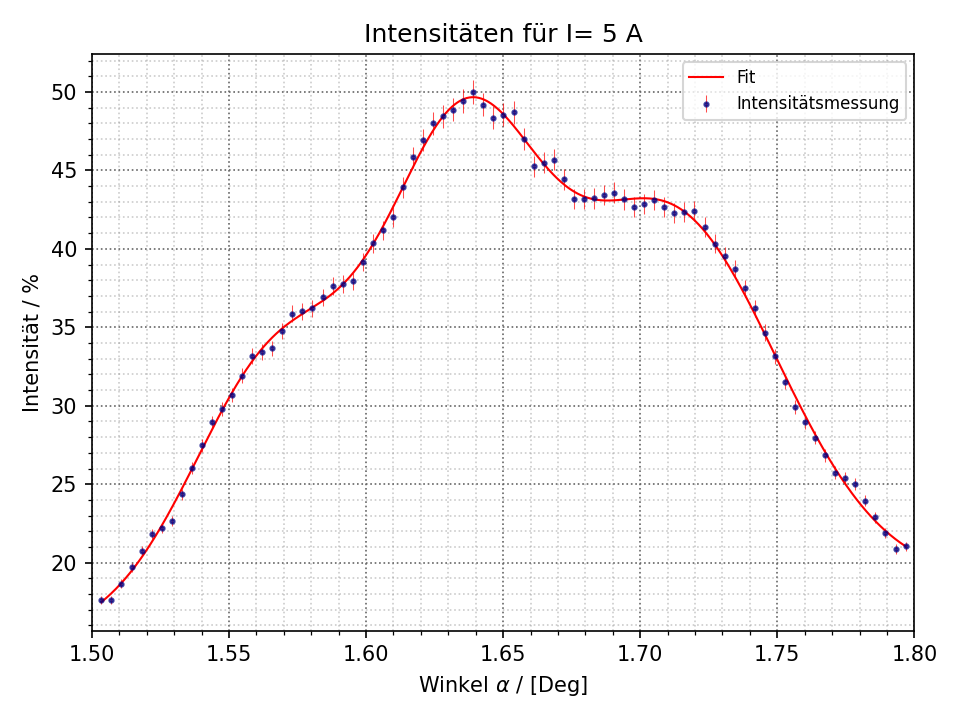
\includegraphics[width=.5\textwidth]{plots/peak_5A}}
    \subcaptionbox{Anpassungskurve für $I = \SI{6}{\ampere}$}{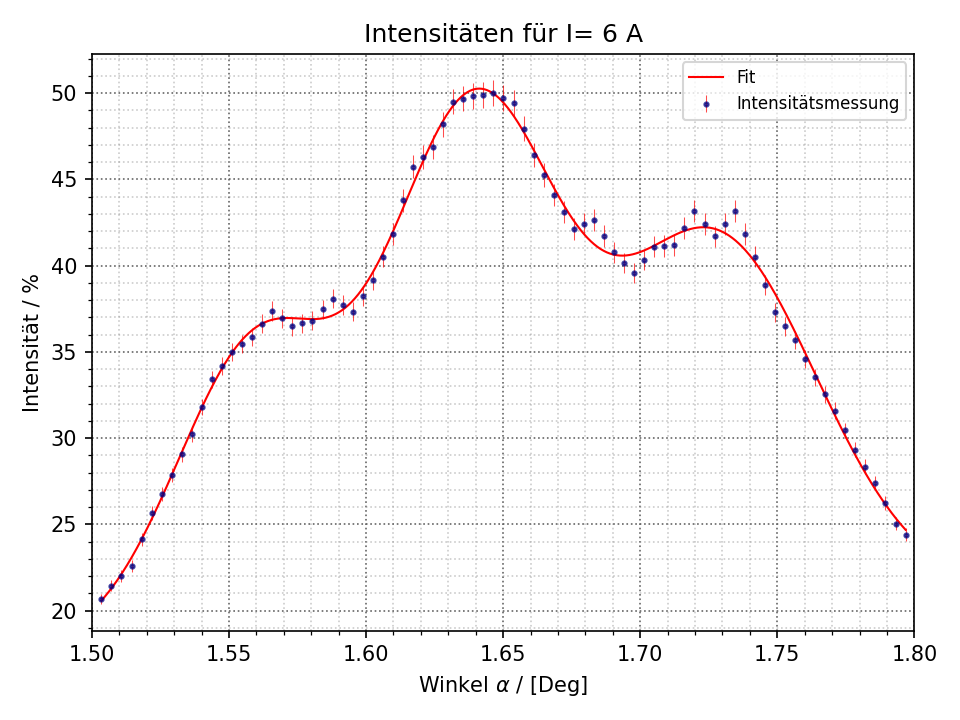
\includegraphics[width=.5\textwidth]{plots/peak_6A}}
    \caption{Mit der \texttt{CCD}-Kamera aufgenommene Intensitätsverläufe im Bereich \\$\alpha \in \left[\SI{1.5}{\degree}\; , \; \SI{1.8}{\degree}\right]$}\label{fig:peaks_all_a}
\end{figure}
\begin{figure}[!ht]
    \subcaptionbox{Anpassungskurve für $I = \SI{7}{\ampere}$}{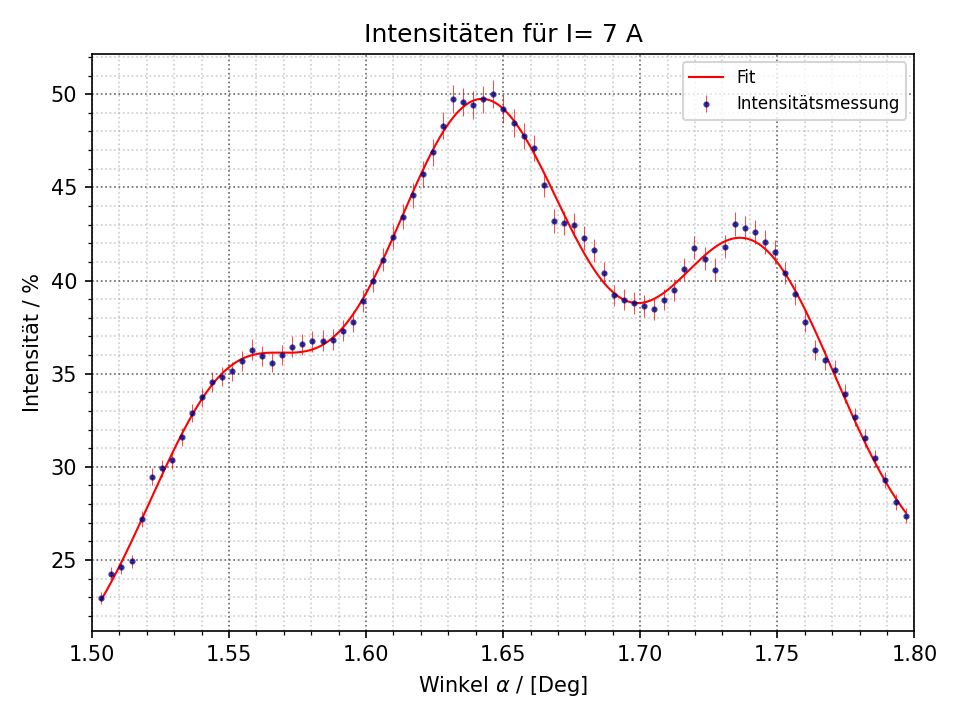
\includegraphics[width=.5\textwidth]{plots/peak_7A}}
    \subcaptionbox{Anpassungskurve für $I = \SI{8}{\ampere}$}{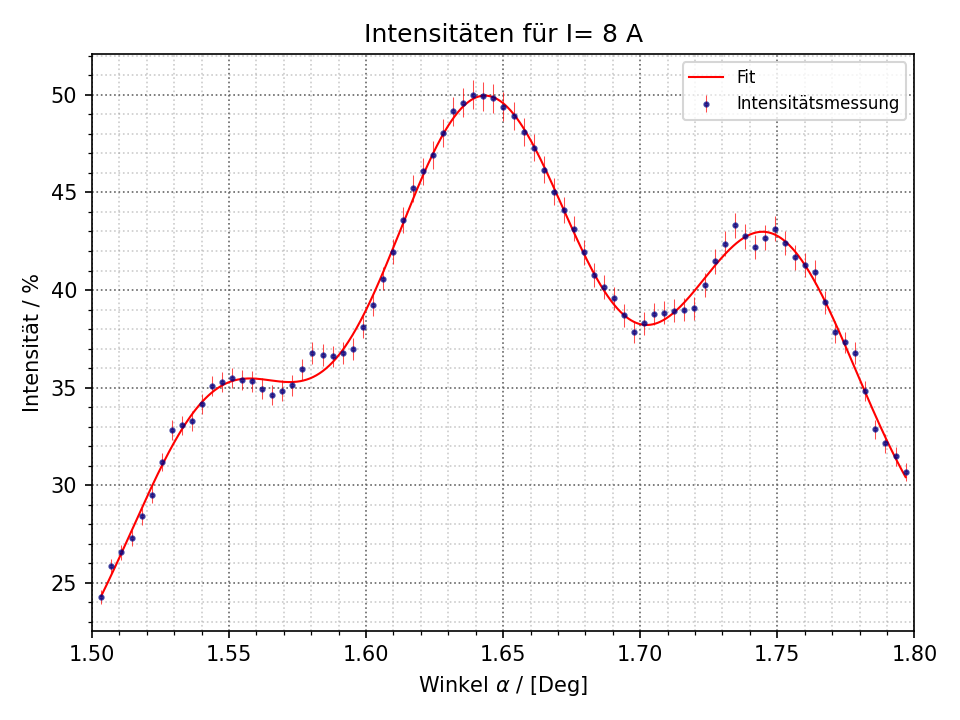
\includegraphics[width=.5\textwidth]{plots/peak_8A}}
    \subcaptionbox{Anpassungskurve für $I = \SI{9}{\ampere}$}{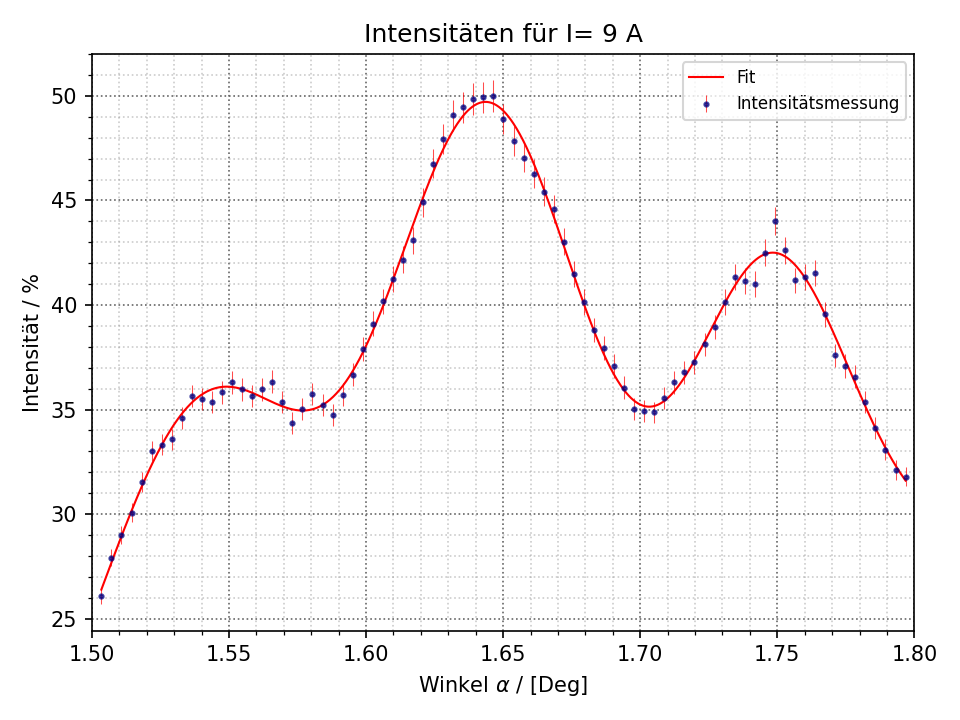
\includegraphics[width=.5\textwidth]{plots/peak_9A}}
    \subcaptionbox{Anpassungskurve für $I = \SI{10}{\ampere}$}{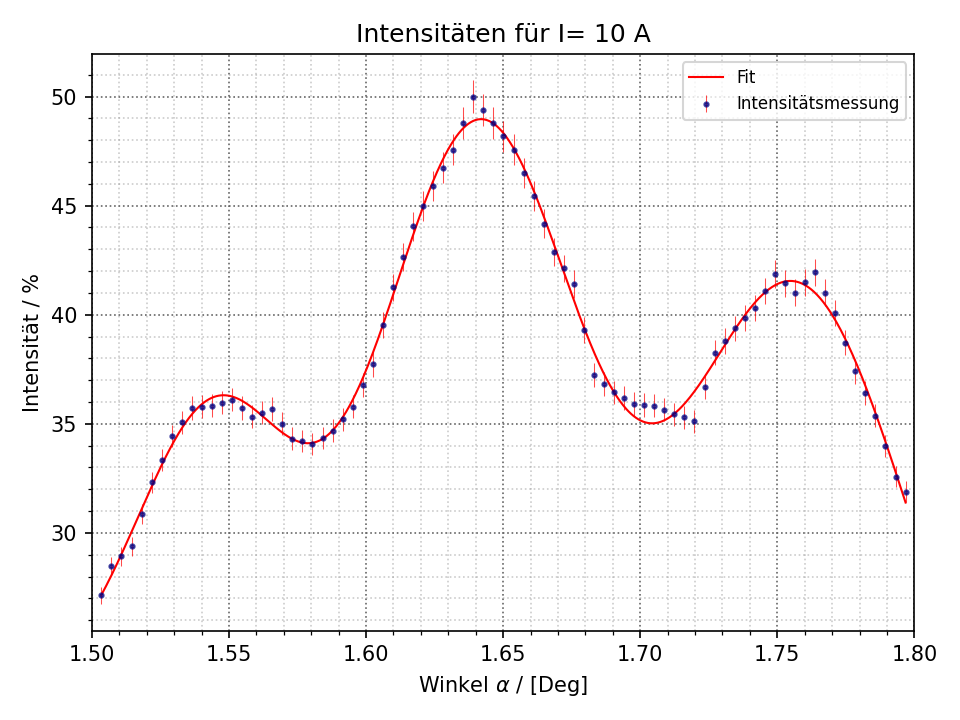
\includegraphics[width=.5\textwidth]{plots/peak_10A}}
    \caption{Mit der \texttt{CCD}-Kamera aufgenommene Intensitätsverläufe im Bereich \\$\alpha \in \left[\SI{1.5}{\degree}\; , \; \SI{1.8}{\degree}\right]$}\label{fig:peaks_all_b}
\end{figure}

%-----------------------------------------------------------------------
%-----------------------------------------------------------------------
%-----------------------------------------------------------------------
\clearpage
\subsection{Franck-Hertz}
\begin{figure}[!ht]
    \centering
    % first row: U1 & U2
    \subcaptionbox{$U_G$ = $\SI{2}{\volt}$ bei $\SI{165}{\celsius}$}{%
      \includegraphics[width=0.48\textwidth]{plots/UG2.png}%
    }
    \subcaptionbox{$U_G$ = $\SI{2.5}{\volt}$ bei $\SI{165}{\celsius}$}{%
      \includegraphics[width=0.48\textwidth]{plots/UG2_5.png}%
    }
  
    \medskip
    % second row: U3 & U4
    \subcaptionbox{$U_G$ = $\SI{3}{\volt}$ bei $\SI{165}{\celsius}$}{%
      \includegraphics[width=0.48\textwidth]{plots/UG3.png}%
    }
    \subcaptionbox{$U_G$ = $\SI{3.5}{\volt}$ bei $\SI{165}{\celsius}$}{%
      \includegraphics[width=0.48\textwidth]{plots/UG3_5.png}%
    }
  
    \medskip
    % third row: U5 & U6
    \subcaptionbox{$U_G$ = $\SI{4}{\volt}$ bei $\SI{165}{\celsius}$}{%
      \includegraphics[width=0.48\textwidth]{plots/UG4.png}%
    }

  \caption{Anodenspannungskurven in Abhängigkeit der Gegenspannung bei konstanter Temperatur von $T$ = $\SI{165}{\celsius}$.}
    \label{fig:UGall}
\end{figure}

\begin{figure}[!ht]
    \centering
    % first row: U1 & U2
    \subcaptionbox{$T$ = $\SI{165}{\celsius}$ bei $\SI{3}{\volt}$  }{%
      \includegraphics[width=0.48\textwidth]{plots/T165.png}%
    }
    \subcaptionbox{$T$ = $\SI{170}{\celsius}$ bei $\SI{3}{\volt}$}{%
      \includegraphics[width=0.48\textwidth]{plots/T170.png}%
    }
  
    \medskip
    % second row: U3 & U4
    \subcaptionbox{$T$ = $\SI{175}{\celsius}$ bei $\SI{3}{\volt}$}{%
      \includegraphics[width=0.48\textwidth]{plots/T175.png}%
    }
    \subcaptionbox{$T$ = $\SI{180}{\celsius}$ bei $\SI{3}{\volt}$ }{%
      \includegraphics[width=0.48\textwidth]{plots/T180.png}%
    }

  \caption{Anodenspannungskurven in Abhängigkeit der Temperatur bei konstanter Gegenspannung von $U_G$ = $\SI{3}{\volt}$.}
    \label{fig:Tall}
\end{figure}


\clearpage
\section{Tabellen}
\subsection{Zeemann-Effekt}
\begin{table}[ht]
    \centering
    \footnotesize
    \begin{tabular}{c *{5}{c}}
        \toprule
        Parameter & {1} & {2} & {3} & {4} & {5} \\
        \midrule
        $\chi_\text{red}^2$ & 1.34      & 1.68              & 1.11          & 0.72              & 0.83 \\
        $a$         & 2.85 (0.92)       & -8.53 (9.96)      & 9.92 (---)    & 0.043 (1.26)      & 10.96 (2.10) \\
        $b$         & 8.15 (1.43)       & 26.12 (15.02)     & -1.57 (---)   & 17.05 (1.94)      & -0.96 (3.53) \\
        $A_1$       & 0.046 (0.015)     & 0.008 (0.0043)    & 7.1e-7 (---)  & 0.803 (0.077)     & 1.336 (0.185) \\
        $\sigma_1$  & 0.015 (0.0030)    & 0.0049 (0.0025)   & 0.045 (---)   & 0.024 (0.0013)    & 0.031 (0.0024) \\
        $\mu_1$     & 1.559 (0.0029)    & 1.537 (0.0022)    & 1.547 (---)   & 1.573 (0.0022)    & 1.569 (0.0030) \\
        $A_2$       & 3.201 (0.228)     & 4.301 (0.194)     & 4.672 (---)   & 0.831 (0.191)     & 1.835 (0.228) \\
        $\mu_2$     & 1.644 (0.0023)    & 1.649 (0.0009)    & 1.649 (---)   & 1.625 (0.0018)    & 1.635 (0.0014) \\
        $\sigma_2$  & 0.0349 (0.0012)   & 0.0453 (0.0008)   & 0.0533 (---)  & 0.0229 (0.0021)   & 0.0279 (0.0017) \\
        $A_3$       & 0.488 (0.243)     & 0.575 (0.376)     & 0.146 (---)   & 3.705 (0.235)     & 2.473 (0.194) \\
        $\mu_3$     & 1.711 (0.013)     & 1.761 (0.0087)    & 1.725 (---)   & 1.682 (0.0027)    & 1.709 (0.0022) \\
        $\sigma_3$  & 0.0340 (0.0062)   & 0.0426 (0.0100)   & 0.0346 (---)  & 0.0502 (0.0020)   & 0.0403 (0.0020) \\
        \bottomrule
    \end{tabular}
    \vspace{1em}
    \begin{tabular}{c *{5}{c}}
        \toprule
        Parameter & {6} & {7} & {8} & {9} & {10} \\
        \midrule
        $\chi_\text{red}^2$ & 0.858 & 0.825 & 0.620 & 0.674 & 0.669 \\
        $a$         & 10.04 (3.07)      & 18.77 (4.66)      & 22.47 (6.25)      & 46.72 (13.07)     & -21.55 (15.45) \\
        $b$         & 2.92 (4.93)       & -10.10 (8.08)     & -15.89 (10.80)    & -56.16 (23.80)    & 54.46 (22.96) \\
        $A_1$       & 1.223 (0.128)     & 1.183 (0.195)     & 1.226 (0.234)     & 1.896 (0.566)     & 1.029 (0.194) \\
        $\sigma_1$  & 0.0293 (0.0017)   & 0.0312 (0.0025)   & 0.0325 (0.0027)   & 0.0387 (0.0043)   & 0.0288 (0.0022) \\
        $\mu_1$     & 1.560 (0.0015)    & 1.551 (0.0014)    & 1.546 (0.0012)    & 1.541 (0.0019)    & 1.545 (0.0010) \\
        $A_2$       & 2.263 (0.117)     & 2.608 (0.0833)    & 2.692 (0.105)     & 2.509 (0.207)     & 2.673 (0.259) \\
        $\mu_2$     & 1.639 (0.00087)   & 1.641 (0.00074)   & 1.642 (0.00057)   & 1.643 (0.00091)   & 1.642 (0.00051) \\
        $\sigma_2$  & 0.0311 (0.0014)   & 0.0364 (0.0014)   & 0.0375 (0.0010)   & 0.0351 (0.0007)   & 0.0363 (0.0008) \\
        $A_3$       & 2.010 (0.188)     & 1.542 (0.155)     & 1.578 (0.189)     & 1.202 (0.151)     & 2.541 (0.716) \\
        $\mu_3$     & 1.727 (0.0015)    & 1.739 (0.0010)    & 1.746 (0.00086)   & 1.747 (0.00078)   & 1.758 (0.0018) \\
        $\sigma_3$  & 0.0375 (0.0021)   & 0.0325 (0.0017)   & 0.0331 (0.0018)   & 0.0288 (0.0015)   & 0.0410 (0.0042) \\
        \bottomrule
    \end{tabular}
    \caption[Anpassungsparameter zur Messreihe \textsc{Zeeman}-Effekt]{Anpassungsparameter der Gaußkurven aus der Messreihe zum \textsc{Zeeman}-Effekt. Die dazugehörigen Abbildungen sind \crefrange{fig:peaks_all_a}{fig:peaks_all_b} zu finden.}\label{tab:langzeeman-fit}
\end{table}
\normalsize
%-----------------------------------------------------------------------
%-----------------------------------------------------------------------
%-----------------------------------------------------------------------
\subsection{Franck-Hertz}
\begin{table}[h!]
    \centering
    \sisetup{uncertainty-mode=separate}
    \begin{tabular}{
      l|
      S[table-format=1.3(3)]
      S[table-format=1.3(3)]
    }
    \toprule
    \multicolumn{1}{c|}{$U_G$ [V] (bei Temperatur = $\SI{165}{\degreeCelsius}$)} &
    \multicolumn{1}{c}{$\Delta E$ [eV]} &
    \multicolumn{1}{c}{$\sigma$ [V]} \\
    \midrule
    2.0 & 4.830 \pm 0.183 & 0.817 \pm 0.328 \\
    2.5 & 4.810 \pm 0.220 & 0.921 \pm 0.107 \\
    3.0 & 4.830 \pm 0.320 & 0.903 \pm 0.085 \\
    3.5 & 4.840 \pm 0.260 & 0.862 \pm 0.082 \\
    4.0 & 4.850 \pm 0.207 & 0.635 \pm 0.300 \\
    \bottomrule
    \end{tabular}
    \caption{Gemittelte $\Delta E$ und Breite der angepassten Gaußkurven für jede Gegenspannung}
    \label{tab:franckU2}
  \end{table}
  \vspace{1em}
  \begin{table}[h!]
    \centering
    \sisetup{uncertainty-mode=separate}
    \begin{tabular}{
      l|
      S[table-format=1.3(3)]
      S[table-format=1.3(3)]
    }
    \toprule
    \multicolumn{1}{c|}{Temperatur [\si{\degreeCelsius}] (bei $U_G$ = $3 \si{\volt}$)} &
    \multicolumn{1}{c}{$\Delta E$ [eV]} &
    \multicolumn{1}{c}{$\sigma$ [V]} \\
    \midrule
    165 & 4.840 \pm 0.193 & 0.911 \pm 0.074 \\
    170 & 4.830 \pm 0.183 & 0.917 \pm 0.065 \\
    175 & 4.800 \pm 0.158 & 0.927 \pm 0.061 \\
    180 & 4.810 \pm 0.037 & 0.900 \pm 0.080 \\
    \bottomrule
    \end{tabular}
    \caption{Gemittelte $\Delta E$ und Breite der angepassten Gaußkurven für jede Temperatur}
    \label{tab:franckT}
  \end{table}
  
  

\end{document}